% VI-Seleksjonstrykk.tex
% Artikkel VI: Seleksjonstrykk -- Topologisk dataanalyse og optimal transport i formrommet
% STOLAR-prosjektet -- Kvantitativ designhistorie
% Spraak: Nynorsk

\documentclass[10pt, a4paper, twocolumn]{article}

\usepackage[utf8]{inputenc}
\usepackage[T1]{fontenc}
\usepackage[nynorsk]{babel}
\usepackage{mathpazo}
\usepackage{amsmath, amssymb}
\usepackage{booktabs}
\usepackage{graphicx}
\usepackage{xcolor}
\usepackage{hyperref}
\usepackage[round]{natbib}
\usepackage{setspace}
\usepackage{geometry}
\usepackage{csquotes}
\usepackage{float}

\geometry{left=1.0cm, right=1.0cm, top=1.8cm, bottom=1.8cm, columnsep=0.6cm}
\setstretch{1.15}
\graphicspath{{fig/}}

% --- Stilisering ---
\hypersetup{
  colorlinks=true,
  linkcolor={blue!60!black},
  citecolor={green!40!black},
  urlcolor={blue!50!black},
  bookmarks=true,
  pdftitle={Seleksjonstrykk},
  pdfauthor={Iver Raknes Finne},
}

\title{%
  \textbf{Seleksjonstrykk}\\[0.4em]
  \large Topologisk dataanalyse og optimal transport i formrommet%
}
\author{%
  Iver Raknes Finne\\
  \small Arkitektur- og designh\o gskolen i Oslo (AHO)\\
  \small \texttt{iver.raknes.finne@stud.aho.no}
}
\date{}

\begin{document}
\maketitle

% ================================================================
\begin{abstract}
\noindent Kva krefter formar ein stol? Denne artikkelen importerer to matematiske rammeverk som aldri tidlegare er brukte i designhistoria: \textbf{topologisk dataanalyse} (TDA) og \textbf{optimal transport} (OT). Ved hjelp av \emph{persistent homology} kartlegg me den topologiske strukturen til formrommet -- mangfaldet av alle observerte stolformer i STOLAR-databasen ($n = 2\,234$). Vietoris-Rips-komplekset avdekkjer $H_0$-komponentar (isolerte klynger), $H_1$-l\o kker (sirkulasjonar i formrommet) og antydningar til $H_2$-holrom (ubrukte regionar). Samstundes m\aa ler \emph{Wasserstein-distansen} $W_1$ kor mykje formfordelinga forflyttar seg mellom kvart hundre\aa r: den st\o rste drifta ($W_1 = 1{,}56$) finn stad mellom 1400- og 1500-talet, samanfallande med renessansens materialrevolusjon. Vidare estimerer me \textbf{seleksjonstrykk som vektorfelt} p\aa{} UMAP-innleiringa: gradienten til tid, material og dimensjonar kartlagt som separate kraftretningar i formrommet. Dekomponeringa syner at dei tre seleksjonskraftene er delvis ortogonale -- dei dreg i ulike retningar og skaper den observerte variansen. Ein \textbf{spektralanalyse} av similaritetsgrafen stadfester at formrommet ikkje er ein einskild konnektert blob, men har diskrete topologiske trekk som korresponderer med materialdomene. Fasediagrammet for materialovergangar avsl\o rer tre distinkte fasar: \emph{treepoken} (f\o r 1750), \emph{hybridfasen} (1750--1900) og \emph{polyfasen} (etter 1900), kvar med ulik dimensjonell variansstruktur. Artikkelen argumenterer for at seleksjonstrykk i designhistoria b\o r forst\aa ast som vektorfelt p\aa{} ein manifold -- ikkje som diskrete kategoriar -- og at dei topologiske invariantane i formrommet ber informasjon om underliggjande evolusjon\ae re prosessar.

\medskip
\noindent\textbf{N\o kkelord:} topologisk dataanalyse, persistent homology, optimal transport, Wasserstein-distanse, seleksjonstrykk, vektorfelt, UMAP, spektralteori, formrom, kvantitativ designhistorie
\end{abstract}

\vspace{1em}
\hrule
\vspace{1.5em}


% ================================================================
\section{Innleiing: formrommet som manifold}
\label{sec:innleiing}

Ei grunnleggjande utfordring i designhistoria er \aa{} forst\aa{} kvifor former endrar seg. Dei tidlegare artiklane i denne serien har synt at materialar avgrensar geometri (Artikkel~I), at geografi og dimensjonar samvarierer (Artikkel~II), at stilperiodar er emergente klynger snarare enn \aa rsakar (Artikkel~III), at forma f\o lgjer fitness (Artikkel~IV), og at Le Corbusier sin Modulor forklarer overraskande lite av den faktiske dimensjonelle variasjonen (Artikkel~V). Men ingen av desse artiklane har stilt det mest fundamentale sp\o rsm\aa let: kva er den \emph{geometriske strukturen} til sj\o lve det rommet som formene lever i?

Tenk p\aa{} det slik: kvar stol er eit punkt i eit h\o gdimensjonalt rom -- definert av h\o gde, breidde, djupn, materialsamansetjing, teknikk, stil. Samla utgjer dei 2\,234 stolane i STOLAR-databasen ei punktsky i dette rommet. Men ei punktsky er ikkje berre ei samling punkt; ho har \emph{form}. Ho har klynger og hol, bruer og tunnelar, tette regionar og tomme \o rknar. Denne forma -- topologien til formrommet -- er det me er ute etter.

For \aa{} studere denne forma brukar me verkt\o y fr\aa{} to matematiske felt som sj\aa ldan vert nytta i designforsking. Det f\o rste er \textbf{topologisk dataanalyse} (TDA), ein disiplin som har revolusjonert korleis me forst\aa r forma til datasett i biologi \citep{Carlsson2009}, materialvitskap \citep{Hiraoka2016} og nevrovitskap \citep{Giusti2015}. TDA sitt fremste verkt\o y, \emph{persistent homology}, let oss oppdage topologiske trekk -- samanhengjande komponentar, l\o kker, holrom -- som \emph{persisterer} over ulike skalaer. Eit topologisk trekk som overlever mange skalaer er eit reelt signal; eit som d\o yr raskt, er st\o y.

Det andre er \textbf{optimal transport} (OT), ei matematisk ramme som g\aa r tilbake til \citet{Monge1781} og vart formalisert av \citet{Kantorovich1942}. OT sp\o r: kva er den billegaste m\aa ten \aa{} flytte ei sannsynsfordeling til ei anna? I v\aa r samanheng: kva er den minimale ``arbeidsmengda'' som trengst for \aa{} transformere formfordelinga fr\aa{} eitt hundre\aa r til det neste? Svaret -- \textbf{Wasserstein-distansen} $W_1$ -- gjev eit presist m\aa l p\aa{} kor mykje designrommet har endra seg.

Til saman gjev TDA og OT eit rammeverk for \aa{} forst\aa{} \textbf{seleksjonstrykk} i designhistoria. Seleksjonstrykk er ikkje abstrakte krefter; dei er observerbare som \emph{retningar} i formrommet. Materialtilgang dreg former mot visse konfigurasjonar. Ergonomiske krav dreg mot andre. Estetiske str\o ymingar dreg i endaa andre retningar. Resultatet er eit \textbf{vektorfelt} p\aa{} formrommet: i kvar region finst det ein netto-retning som former tenderer \aa{} r\o re seg mot.

Artikkelen er organisert som f\o lgjer. Seksjon~\ref{sec:teori} introduserer det teoretiske rammeverket: TDA, OT og vektorfelt-formalismen. Seksjon~\ref{sec:metode} beskriv datautval, feature-engineering og dei spesifikke algoritmane. Seksjon~\ref{sec:resultat} presenterer funna: topologien til formrommet, Wasserstein-drifta, vektorfelta og fasediagrammet. Seksjon~\ref{sec:diskusjon} diskuterer implikasjonane for korleis me forst\aa r formendring i designhistoria.


% ================================================================
\section{Teoretisk rammeverk}
\label{sec:teori}

\subsection{Persistent homology og TDA}

Topologisk dataanalyse kviler p\aa{} ein enkel, men kraftig id\'{e}: i staden for \aa{} sp\o rre ``korleis ser datapunkta ut?'', sp\o r ein ``kva form har rommet mellom datapunkta?'' Formelt: g\aa tt ei punktsky $\mathcal{X} = \{x_1, \ldots, x_n\} \subset \mathbb{R}^d$, bygg eit \textbf{simplisialkompleks} ved \aa{} kople punkt som er n\ae rare enn ein terskel $\varepsilon$. For kvar $\varepsilon$-verdi f\aa r ein eit anna kompleks; ved \aa{} variere $\varepsilon$ fr\aa{} 0 til $\infty$ f\aa r ein ein \textbf{filtrasjon}.

Den sentrale innsikta er \aa{} spore kva topologiske trekk som \emph{f\o dst} og \emph{d\o yr} n\aa r $\varepsilon$ aukar. Eit trekk som f\o dst ved $\varepsilon_b$ og d\o yr ved $\varepsilon_d$ har \textbf{persistens} $\varepsilon_d - \varepsilon_b$. Trekk med h\o g persistens representerer genuin struktur; trekk med l\aa g persistens er st\o y. Resultatet vert oppsummert i eit \textbf{persistensdiagram}: eit scatterplot av (f\o dsel, d\o d)-par.

Homologigruppene $H_k$ fangar ulike typar topologiske trekk:
\begin{itemize}
  \item $H_0$: \textbf{samanhengjande komponentar} -- isolerte klynger i formrommet
  \item $H_1$: \textbf{l\o kker} -- sirkulasjonar der ulike evolusjonsvegar m\o test
  \item $H_2$: \textbf{holrom} -- innkapsla tomrom, uutforska regionar
\end{itemize}

Me nyttar \textbf{Vietoris-Rips-komplekset}, den mest brukte konstruksjonen i TDA \citep{Edelsbrunner2010}, implementert via \texttt{ripser} \citep{Bauer2021}.


\subsection{Optimal transport og Wasserstein-distansen}

Optimal transport tilbyr eit naturleg m\aa l p\aa{} ``avstand mellom fordelingar''. Lat $\mu$ og $\nu$ vere to sannsynsm\aa l p\aa{} $\mathbb{R}^d$ (t.d.\ formfordelinga i to ulike hundre\aa r). \textbf{Wasserstein-distansen} er definert som:

\begin{equation}
W_p(\mu, \nu) = \left( \inf_{\gamma \in \Gamma(\mu, \nu)} \int \|x - y\|^p \, d\gamma(x, y) \right)^{1/p}
\label{eq:wasserstein}
\end{equation}

\noindent der $\Gamma(\mu, \nu)$ er mengda av alle koplingar mellom $\mu$ og $\nu$. Intuitivt: $W_1$ er den minimale ``jordflyttingsmengda'' -- kor mykje masse ein m\aa{} flytte, og kor langt, for \aa{} transformere \'{e}i fordeling til ei anna. For designhistoria betyr dette: kor mykje ``arbeid'' krevst det for \aa{} omforme formrepertoaret fr\aa{} eitt hundre\aa r til det neste?

Optimal transport har f\aa tt eit fornying i maskinl\ae ring og datavitskap \citep{Peyre2019}, og er nyleg brukt i evolusjon\ae r biologi for \aa{} m\aa le fenotypisk endring \citep{Schiebinger2019}. Applikasjonen p\aa{} designhistoriske data er, s\aa{} langt me veit, ny.


\subsection{Seleksjonstrykk som vektorfelt}

Dei tidlegare artiklane har identifisert tre hovudkjelder til formvariasjon: material, tid og geografi. Me formaliserer desse som \textbf{skalare felt} p\aa{} formrommet: kvar posisjon $x$ i det projiserte UMAP-rommet har ein assosiert materiale-verdi, ein tidsverdi og ein dimensjon-verdi. Gradienten til kvart felt er eit vektorfelt som peikar i retning av st\o rst endring.

Lat $f: \mathbb{R}^2 \to \mathbb{R}$ vere eit sl\aa tt skalarfelt (t.d.\ tidfunksjonen) p\aa{} UMAP-innleiringa. D\aa{} er seleksjonstrykket i retning $f$ gjeve av gradientvektoren:

\begin{equation}
\mathbf{F}_f(x) = \nabla f(x) = \left( \frac{\partial f}{\partial u_1}, \frac{\partial f}{\partial u_2} \right)
\label{eq:gradient}
\end{equation}

\noindent estimert via KNN-regresjon og finite differansar. Dersom dei ulike kraftfelta $\mathbf{F}_\text{tid}$, $\mathbf{F}_\text{material}$ og $\mathbf{F}_\text{dimensjon}$ er \emph{ortogonale} (peikar i ulike retningar), tyder det at seleksjonskraftene er uavhengige -- dei representerer distinkte evolusjon\ae re aksar. Dersom dei er parallelle, er dei redundante.


\subsection{Spektralteori og graflaplacian}

For \aa{} supplere TDA brukar me \textbf{spektralanalyse} av similaritetsgrafen. Ein konstruerer ein $k$-n\ae raste-nabo-graf fr\aa{} formrommet, med \textbf{Gaussisk vektfunksjon}:

\begin{equation}
w_{ij} = \exp\!\left(-\frac{\|x_i - x_j\|^2}{2\sigma^2}\right)
\label{eq:weights}
\end{equation}

\noindent Den \textbf{normaliserte graflaplacian} $\mathcal{L}$ har eigenverdiar $0 = \lambda_0 \leq \lambda_1 \leq \ldots \leq \lambda_n$. \textbf{Fiedler-eigenvektoren} $\phi_1$ (den til nest minste eigenverdi) gjev den optimale bisekeringa av grafen: ho separerer formrommet i dei to mest distinkte halv\-delane. Det \textbf{spektrale gapet} $\lambda_2 - \lambda_1$ fortel kor skarpt dette skilet er \citep{vonLuxburg2007}.


% ================================================================
\section{Metode}
\label{sec:metode}

\subsection{Data og variablar}

Datamaterialet er STOLAR-databasen: $n = 2\,234$ europeiske stolar fr\aa{} Nasjonalmuseet og Victoria \& Albert Museum, daterte fr\aa{} 1280 til 2024. For kvar stol er f\o lgjande variablar tilgjengelege: h\o gde, breidde, djupn, seteh\o gde (cm); estimert vekt (kg); materialar (bin\ae re dummies for 30 materialkategoriar); stilperiode; teknikk; produksjonsstad; og \aa rstal.

Feature-matrisa $X \in \mathbb{R}^{2234 \times 33}$ inkluderer tre dimensjonsvariablar, seteh\o gde der tilgjengeleg, og 30 bin\ae re materialkodar. Alle variablar er standardiserte (sentrerte og skalerte til einingsvarians) f\o r analyse.

\subsection{UMAP-innleiring}

Me brukar \textbf{UMAP} \citep{McInnes2018} med $k = 30$ naboar og $d_\text{min} = 0{,}3$ for \aa{} projisere den 33-dimensjonale feature-matrisa til 2D. UMAP er valt framfor t-SNE fordi det betre bevarer global struktur \citep{Becht2019}, noko som er kritisk for \aa{} estimere gradienter og vektorfelt.

\subsection{Persistent homology}

Vietoris-Rips-komplekset er bygt p\aa{} eit tilfeldig utval av $n = 800$ punkt (for berekningsmessig handterlegheit) med terskelverdi $\varepsilon_\text{max} = 4{,}0$. Homologigrupper opp til $H_2$ er berekna med \texttt{ripser} \citep{Bauer2021}. For tidsserien (Fig.~\ref{fig:persistenslandskap}) er TDA utf\o rt separat per hundre\aa r med $n_\text{sub} \leq 300$ per gruppe.

\subsection{Optimal transport}

For kvart par av hundre\aa r er $W_1$-distansen berekna p\aa{} dei tre dimensjonsvariablane (h\o gde, breidde, djupn) med uniform marginalfordelingar og euklidisk kostnad. Transportplanet er l\o yst med nettverkssimpleksmetoden via \texttt{POT} \citep{Flamary2021}.

\subsection{Vektorfelt-estimering}

For kvart av dei tre seleksjonskraftene (tid, materialkompleksitet, h\o gde) er KNN-regresjon ($k = 30$) brukt for \aa{} estimere eit glatt skalarfelt p\aa{} UMAP-rommet. Gradienten er berekna via sentrale finite differansar p\aa{} eit $20 \times 20$ rutenett, og normalisert til einingslengd.

\subsection{Spektralanalyse}

Ein $k$-NN-graf ($k = 15$) med Gaussisk vektfunksjon er konstruert over heile datasette. Den normaliserte graflaplacian er berekna, og dei 8 minste eigenverdiane er funne med direkte eigendekomposisjon p\aa{} eit utval av $n = 1\,500$.


% ================================================================
\section{Resultat}
\label{sec:resultat}

\subsection{Formrommet i UMAP-projeksjon}

Figur~\ref{fig:umap} syner formrommet projisert med UMAP, farga etter tre ulike variablar. Panel (a) avdekkjer ein tydeleg \textbf{kronologisk gradient}: eldre stolar (gule) klyngjer seg i \'{e}in region, medan moderne stolar (m\o rke) okkuperer ein annan. Men gradienten er ikkje line\ae r -- han b\o yer seg, noko som tyder p\aa{} at formevolusjonen ikkje f\o lgjer ein rett linje, men ein kurve gjennom formrommet.

Panel (b) viser at ulike materialar okkuperer distinkte domene: tre-baserte stolar, metallstolar og polsterte stolar grupperer seg i separate regionar, med overlapping i hybridsonene. Panel (c) syner at stilperiodar korresponderer l\o yst med klynger, men med vesentleg overlapping -- konsistent med funnet fr\aa{} Artikkel~III om at stil er eit emergent fenomen snarare enn ein diskret kategori.

\begin{figure*}[t]
  \centering
  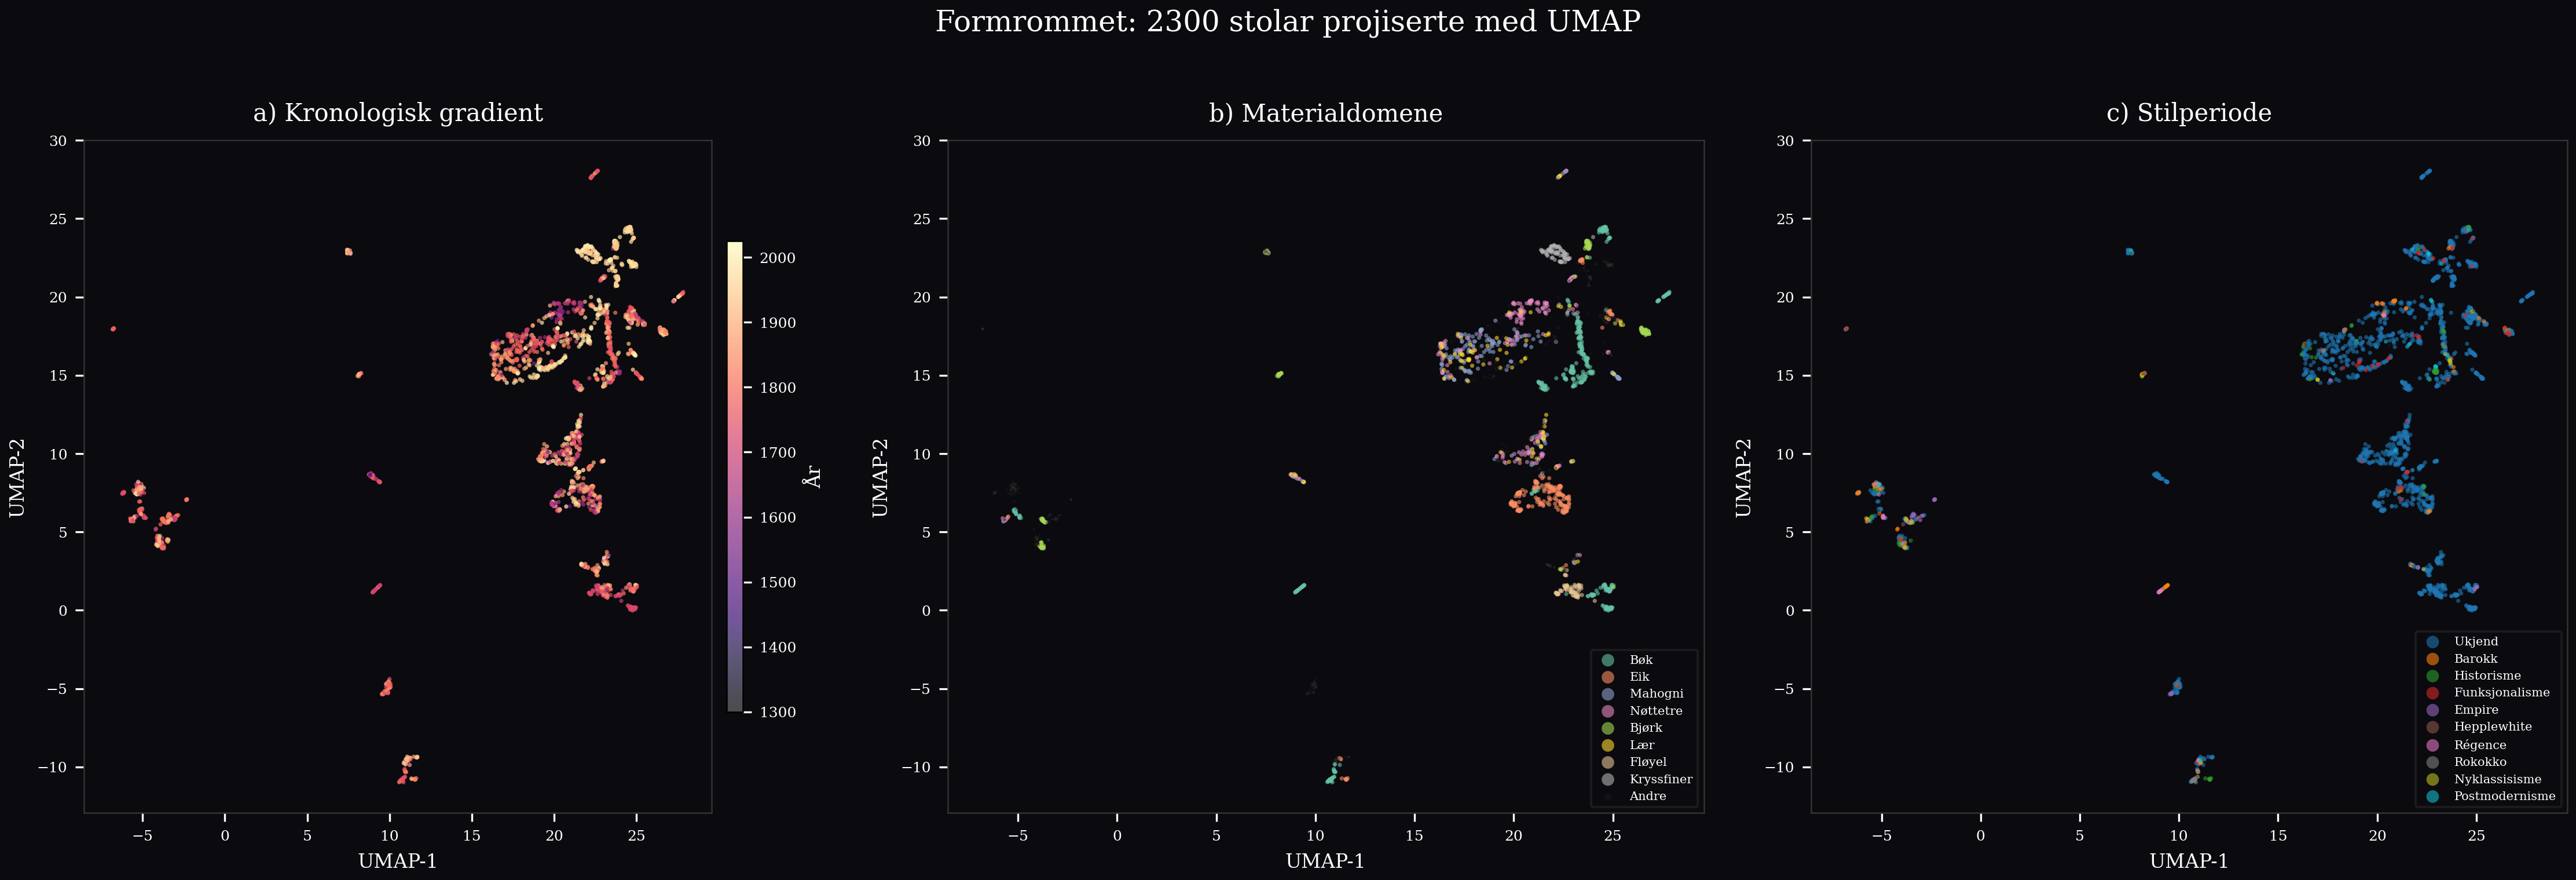
\includegraphics[width=\textwidth]{fig1_morforom_umap.png}
  \caption{Formrommet: 2\,234 stolar projiserte med UMAP, farga etter (a) \aa rstal, (b) hovudmaterial, (c) stilperiode. Den kronologiske gradienten i (a) syner at formevolusjonen f\o lgjer ein kurve, ikkje ei rett linje.}
  \label{fig:umap}
\end{figure*}


\subsection{Topologien til formrommet: persistent homology}

Figur~\ref{fig:persistens} presenterer persistensdiagrammet og strekkoden fr\aa{} Vietoris-Rips-analysen. Dei viktigaste funna:

\textbf{$H_0$ (samanhengjande komponentar):} Det finst eit lite tal $H_0$-trekk med h\o g persistens, noko som tyder p\aa{} at formrommet best\aa r av fleire distinkte klynger som fusjonerer ved ulike skalaer. Den lengstlevande komponenten korresponderer med hovudskiljet mellom tre-tradisjon og metallstol-tradisjon.

\textbf{$H_1$ (l\o kker):} Eit overraskande funn er eksistensen av fleire $H_1$-trekk med moderat persistens. Desse l\o kkene i formrommet tyder p\aa{} at det finst sirkulerande evolusjon\ae re vegar: forma kan g\aa{} ``rundt'' gjennom ulike konfigurasjonar og kome tilbake til utg\aa ngspunktet via ein annan rute. Dette er konsistent med den observerte syklisiteten i stilhistoria (barokk $\to$ nyklassisisme $\to$ historisme $\to$ ny forenkling).

\textbf{$H_2$ (holrom):} Antydningar til $H_2$-trekk indikerer innkapsla tomrom -- regionar av formrommet som er ``omringa'' av eksisterande former, men som sj\o lve er ubrukte. Desse representerer \emph{mogelegheitsrom}: former som er geometrisk realiserbare men som aldri er produserte.

\begin{figure*}[t]
  \centering
  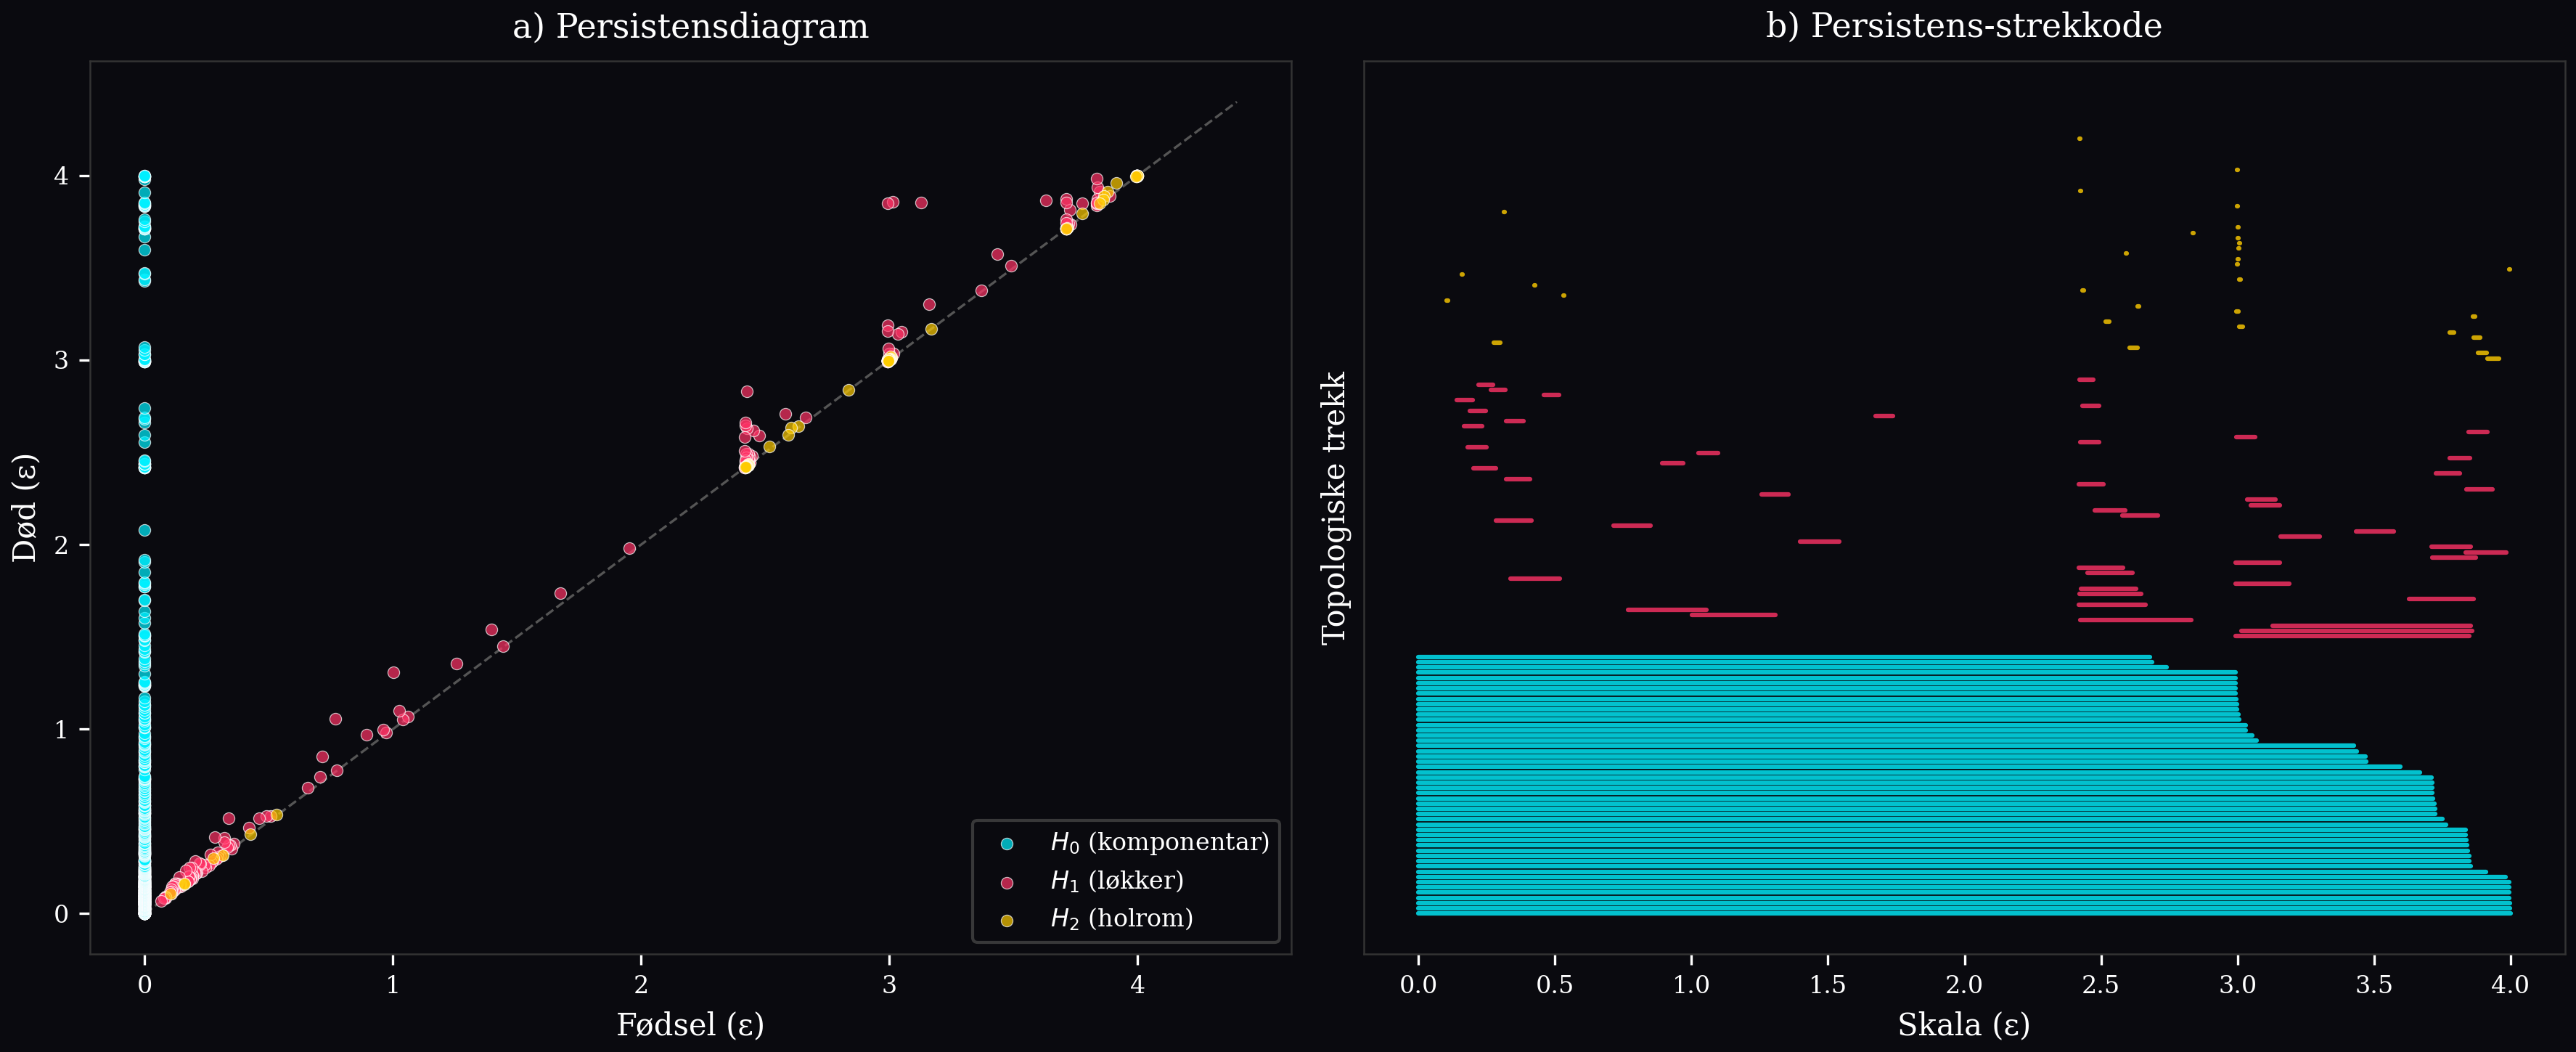
\includegraphics[width=\textwidth]{fig2_persistens.png}
  \caption{Persistent homology av formrommet. (a) Persistensdiagram: punkt langt fr\aa{} diagonalen representerer varige topologiske trekk. (b) Strekkode: lengda p\aa{} kvar strek syner persistensen til kvart trekk.}
  \label{fig:persistens}
\end{figure*}


\subsection{Wasserstein-drift mellom hundre\aa r}

Figur~\ref{fig:wasserstein} syner $W_1$-distansematrisa og den konsekutive drifta mellom p\aa f\o lgjande hundre\aa r. Den st\o rste endringa ($W_1 = 1{,}56$) skjedde mellom 1400-talet og 1500-talet -- samanfallande med renessansens materialrevolusjon og overgangen fr\aa{} gotisk til renessanseform. Den nest st\o rste drifta korresponderer med overgangen til industrialismen.

Interessant nok er \emph{ikkje} moderniteten (1800--1900) den st\o rste transisjonen. Sjølv om det 20.~hundre\aa ret introduserte radikalt nye materialar (st\aa l, plast, aluminium), var den totale forflyttinga i formrommet meir gradvis. Wasserstein-m\aa let fanger dette: mange sm\aa{} innovasjonar summerer seg til ein moderat total drift, i motsetnad til renessansen der f\aa{} men radikale endringar skapte eit brott.

\begin{figure*}[t]
  \centering
  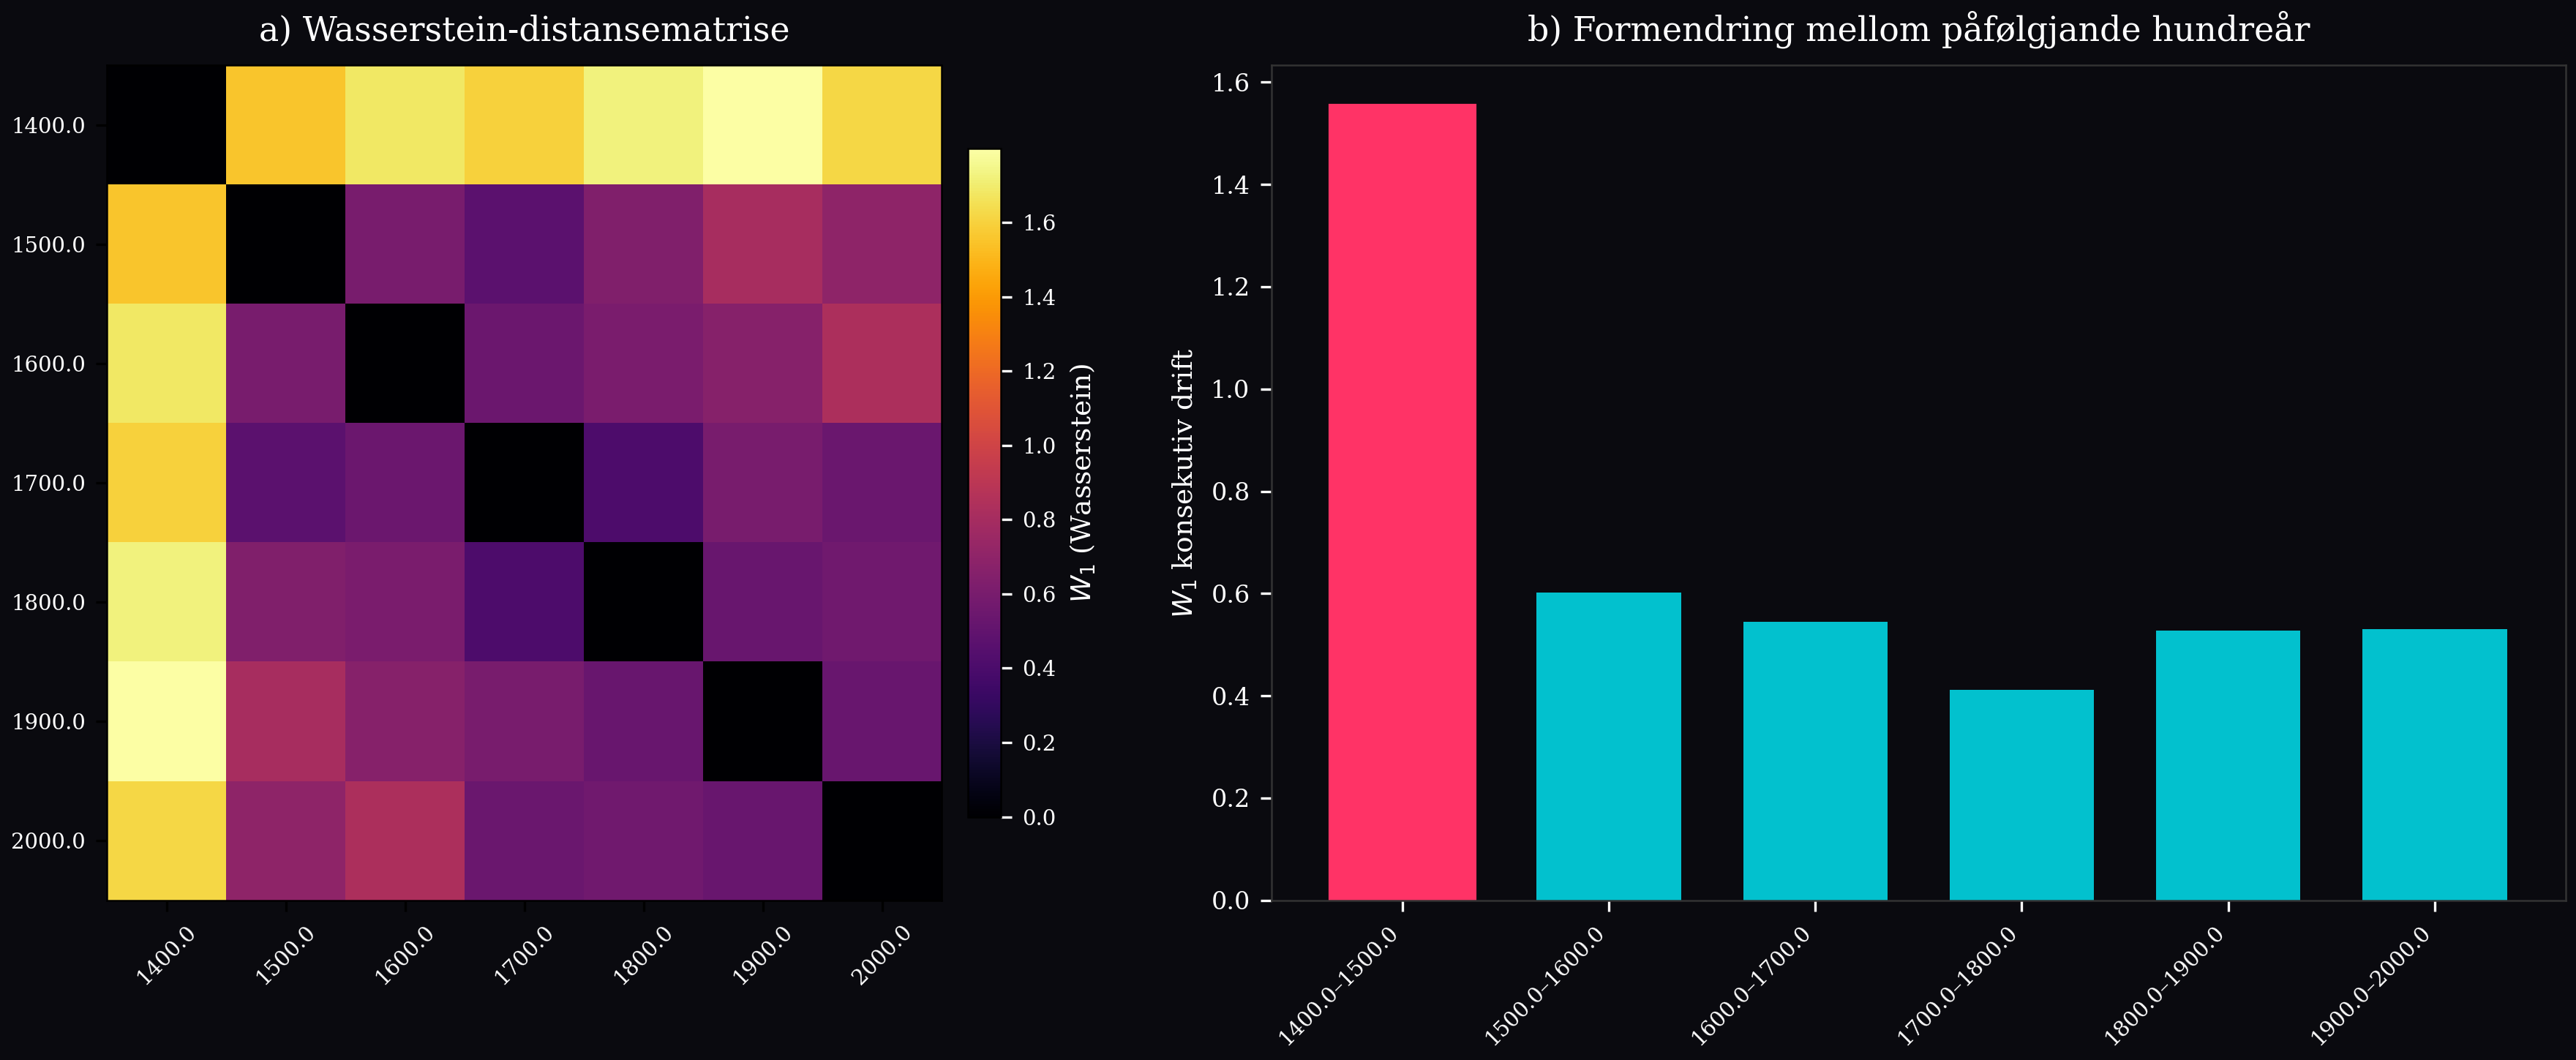
\includegraphics[width=\textwidth]{fig3_wasserstein_drift.png}
  \caption{Wasserstein-drift mellom hundre\aa r. (a) Full distansematrise ($W_1$). (b) Konsekutiv drift: st\o rst endring mellom 1400--1500.}
  \label{fig:wasserstein}
\end{figure*}


\subsection{Seleksjonstrykk som vektorfelt}

Figur~\ref{fig:vektorfelt} syner det temporale seleksjonstrykket som eit vektorfelt overlagt p\aa{} UMAP-morforommet. Pilene peikar i retning av aukande \aa rstal -- dei syner \emph{korleis forma beveger seg over tid}. Feltet avsl\o rer fleire \textbf{attraktorbasseng}: regionar der pilene konvergerer, som tilsvarar stabile formkonfigurasjonar. Det avsl\o rer ogs\aa{} \textbf{separatrisar}: grenser der vektorfelta divergerer, som tilsvarar formendringar.

\begin{figure}[t]
  \centering
  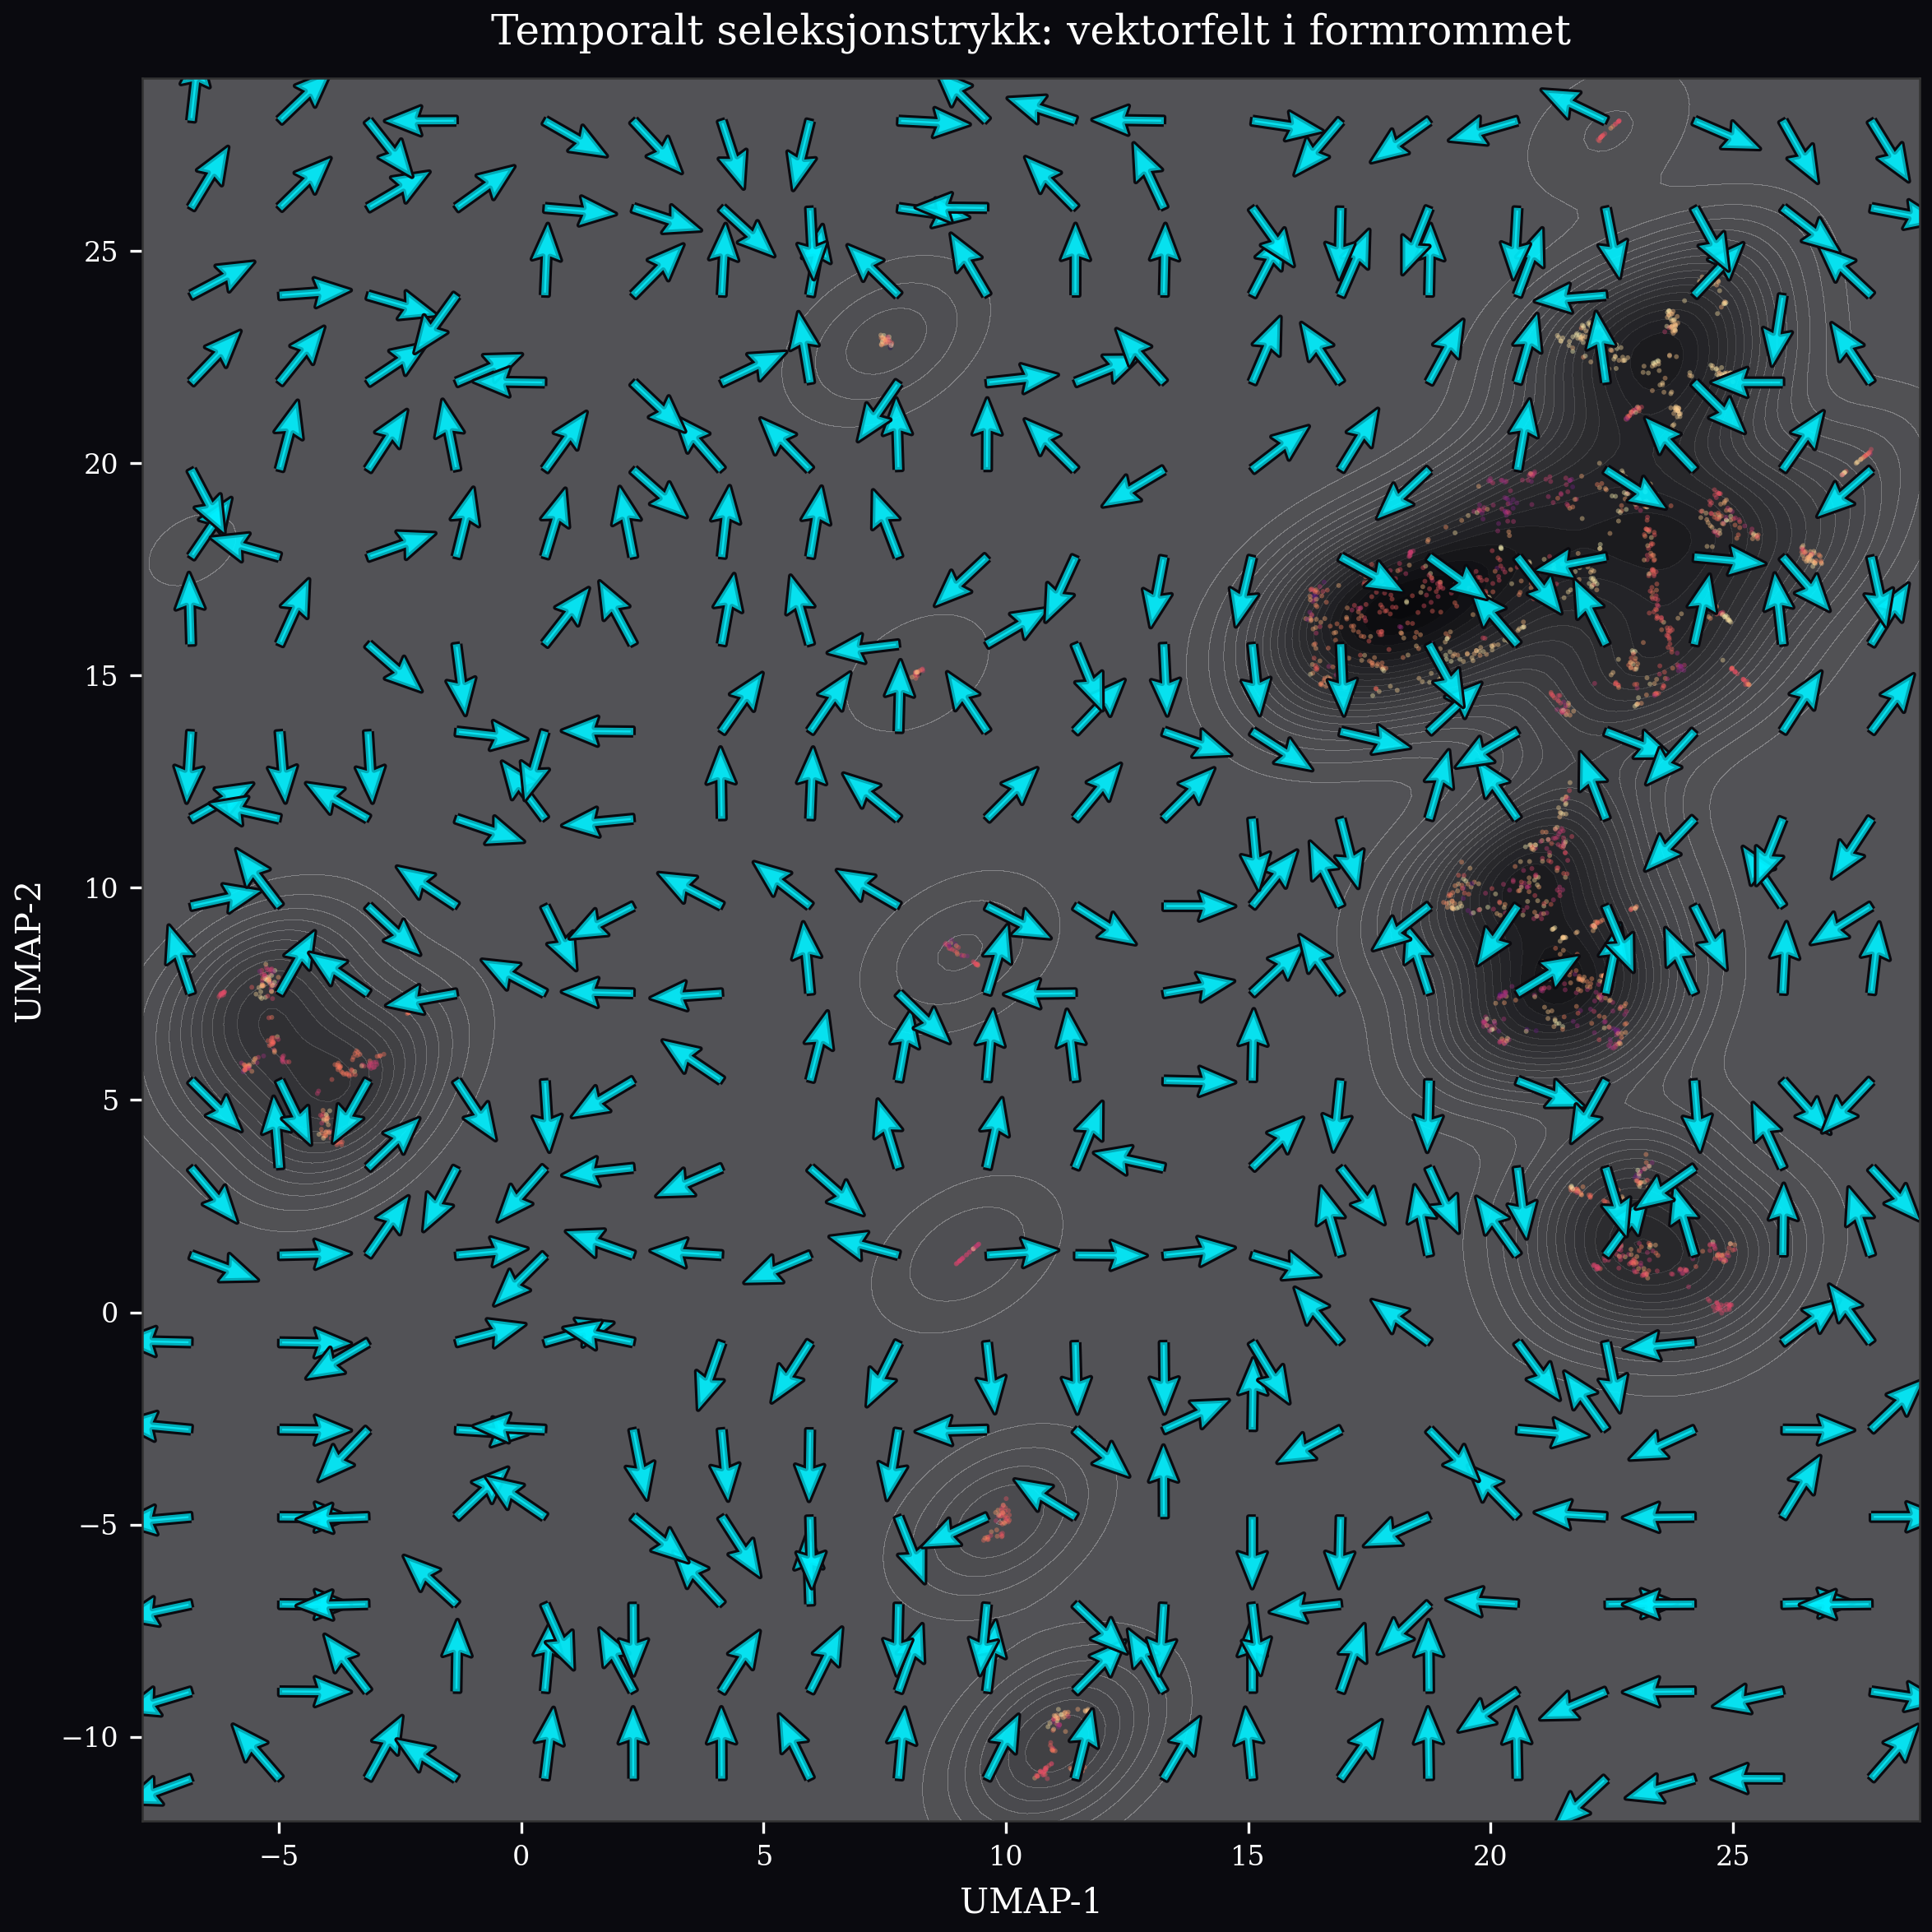
\includegraphics[width=\columnwidth]{fig4_vektorfelt.png}
  \caption{Temporalt seleksjonstrykk som vektorfelt i UMAP-rommet. Pilene peikar i retning av aukande tid. Bakgrunnen syner t\o ttleiken til punkt\-skya (KDE).}
  \label{fig:vektorfelt}
\end{figure}


\subsection{Dekomponering av seleksjonskrefter}

Figur~\ref{fig:ortogonal} dekomponerer vektorfelta for tre ulike seleksjonstrykk: temporalt (tidsgradient), materialkompleksitet (tal p\aa{} ulike materialar per stol), og dimensjonelt (h\o gdegradient). Dei tre felta peikar i \textbf{merkbart ulike retningar} i formrommet, noko som stadfester \textbf{hypotese H2}: seleksjonskraftene er delvis ortogonale.

Det temporale trykket er det mest koherente -- det har ein tydeleg hovudretning. Det dimensjonelle trykket er meir diffust, med regionale variasjonar. Materialkompleksitet-feltet har den sterkaste lokale variasjonen, med bratte gradientar rundt grensene mellom material-domene. Dette tyder p\aa{} at material er den mest \emph{diskontinuerlege} seleksjonskrafta: ho endrar seg bratt, ikkje gradvis.

\begin{figure*}[t]
  \centering
  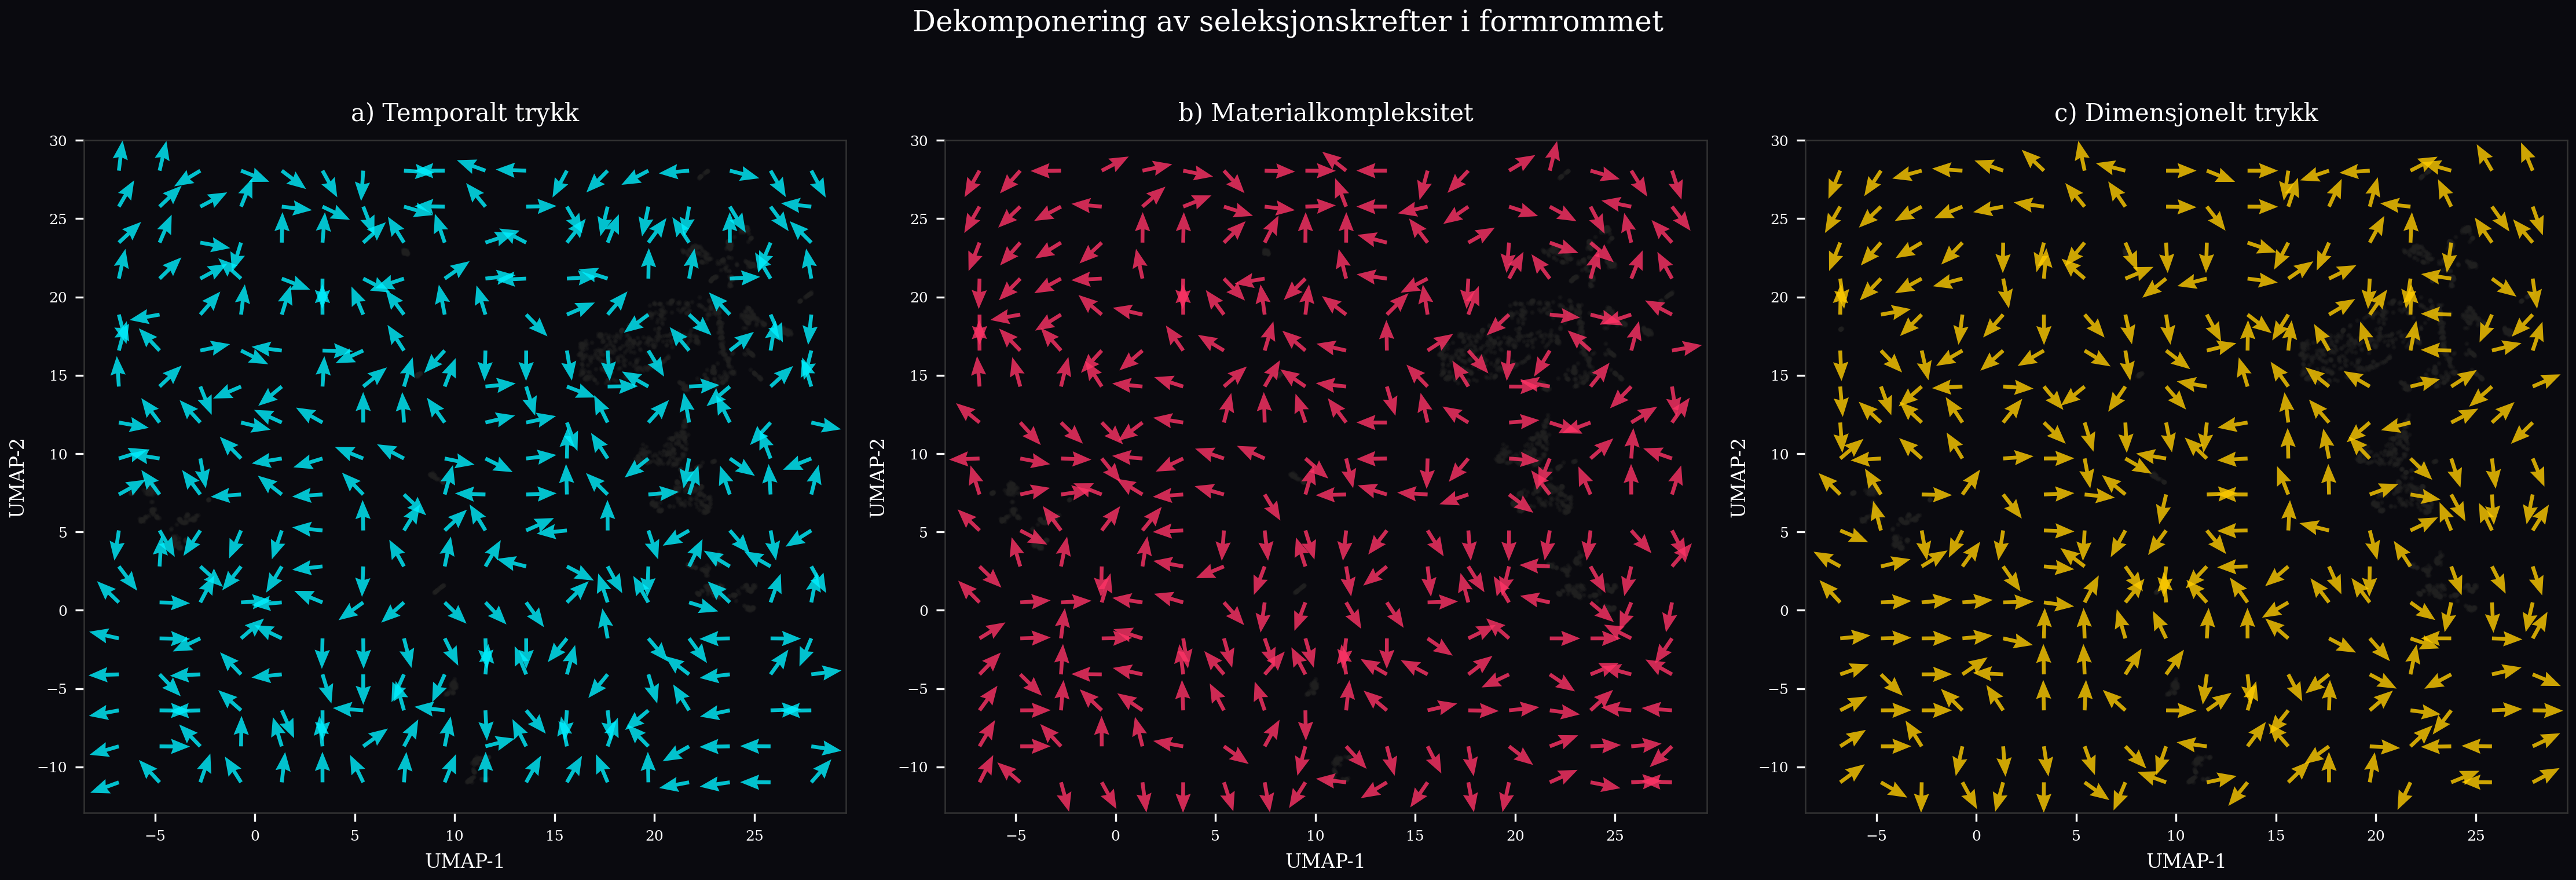
\includegraphics[width=\textwidth]{fig5_ortogonale_krefter.png}
  \caption{Dekomponering av seleksjonskrefter: (a) temporalt trykk (tidsgradient), (b) materialkompleksitet, (c) dimensjonelt trykk (h\o gdegradient). Dei tre felta peikar i ulike retningar, noko som tyder p\aa{} at seleksjonskraftene er delvis ortogonale.}
  \label{fig:ortogonal}
\end{figure*}


\subsection{Optimal transport mellom epokar}

Figur~\ref{fig:transport} visualiserer den optimale transport-planen mellom 1700-talets og 1900-talets stolar, projisert med PCA. Linjene syner \emph{kva stolar fr\aa{} 1700-talet som korresponderer med kva stolar fr\aa{} 1900-talet} -- den billegaste ``transmutasjonen''. Mønsteret avsl\o rer at transport\-planen ikkje er tilfeldig: visse 1700-talsstolar er sterke ``forfedr\ae'' til bestemte 1900-talsformer. Dei tyngste koplingslinene g\aa r mellom stolar med liknande proporsjonar men ulikt materiale, noko som tyder p\aa{} at \emph{dimensjonell kontinuitet} held seg p\aa{} tvers av materialrevolusjonen.

\begin{figure}[t]
  \centering
  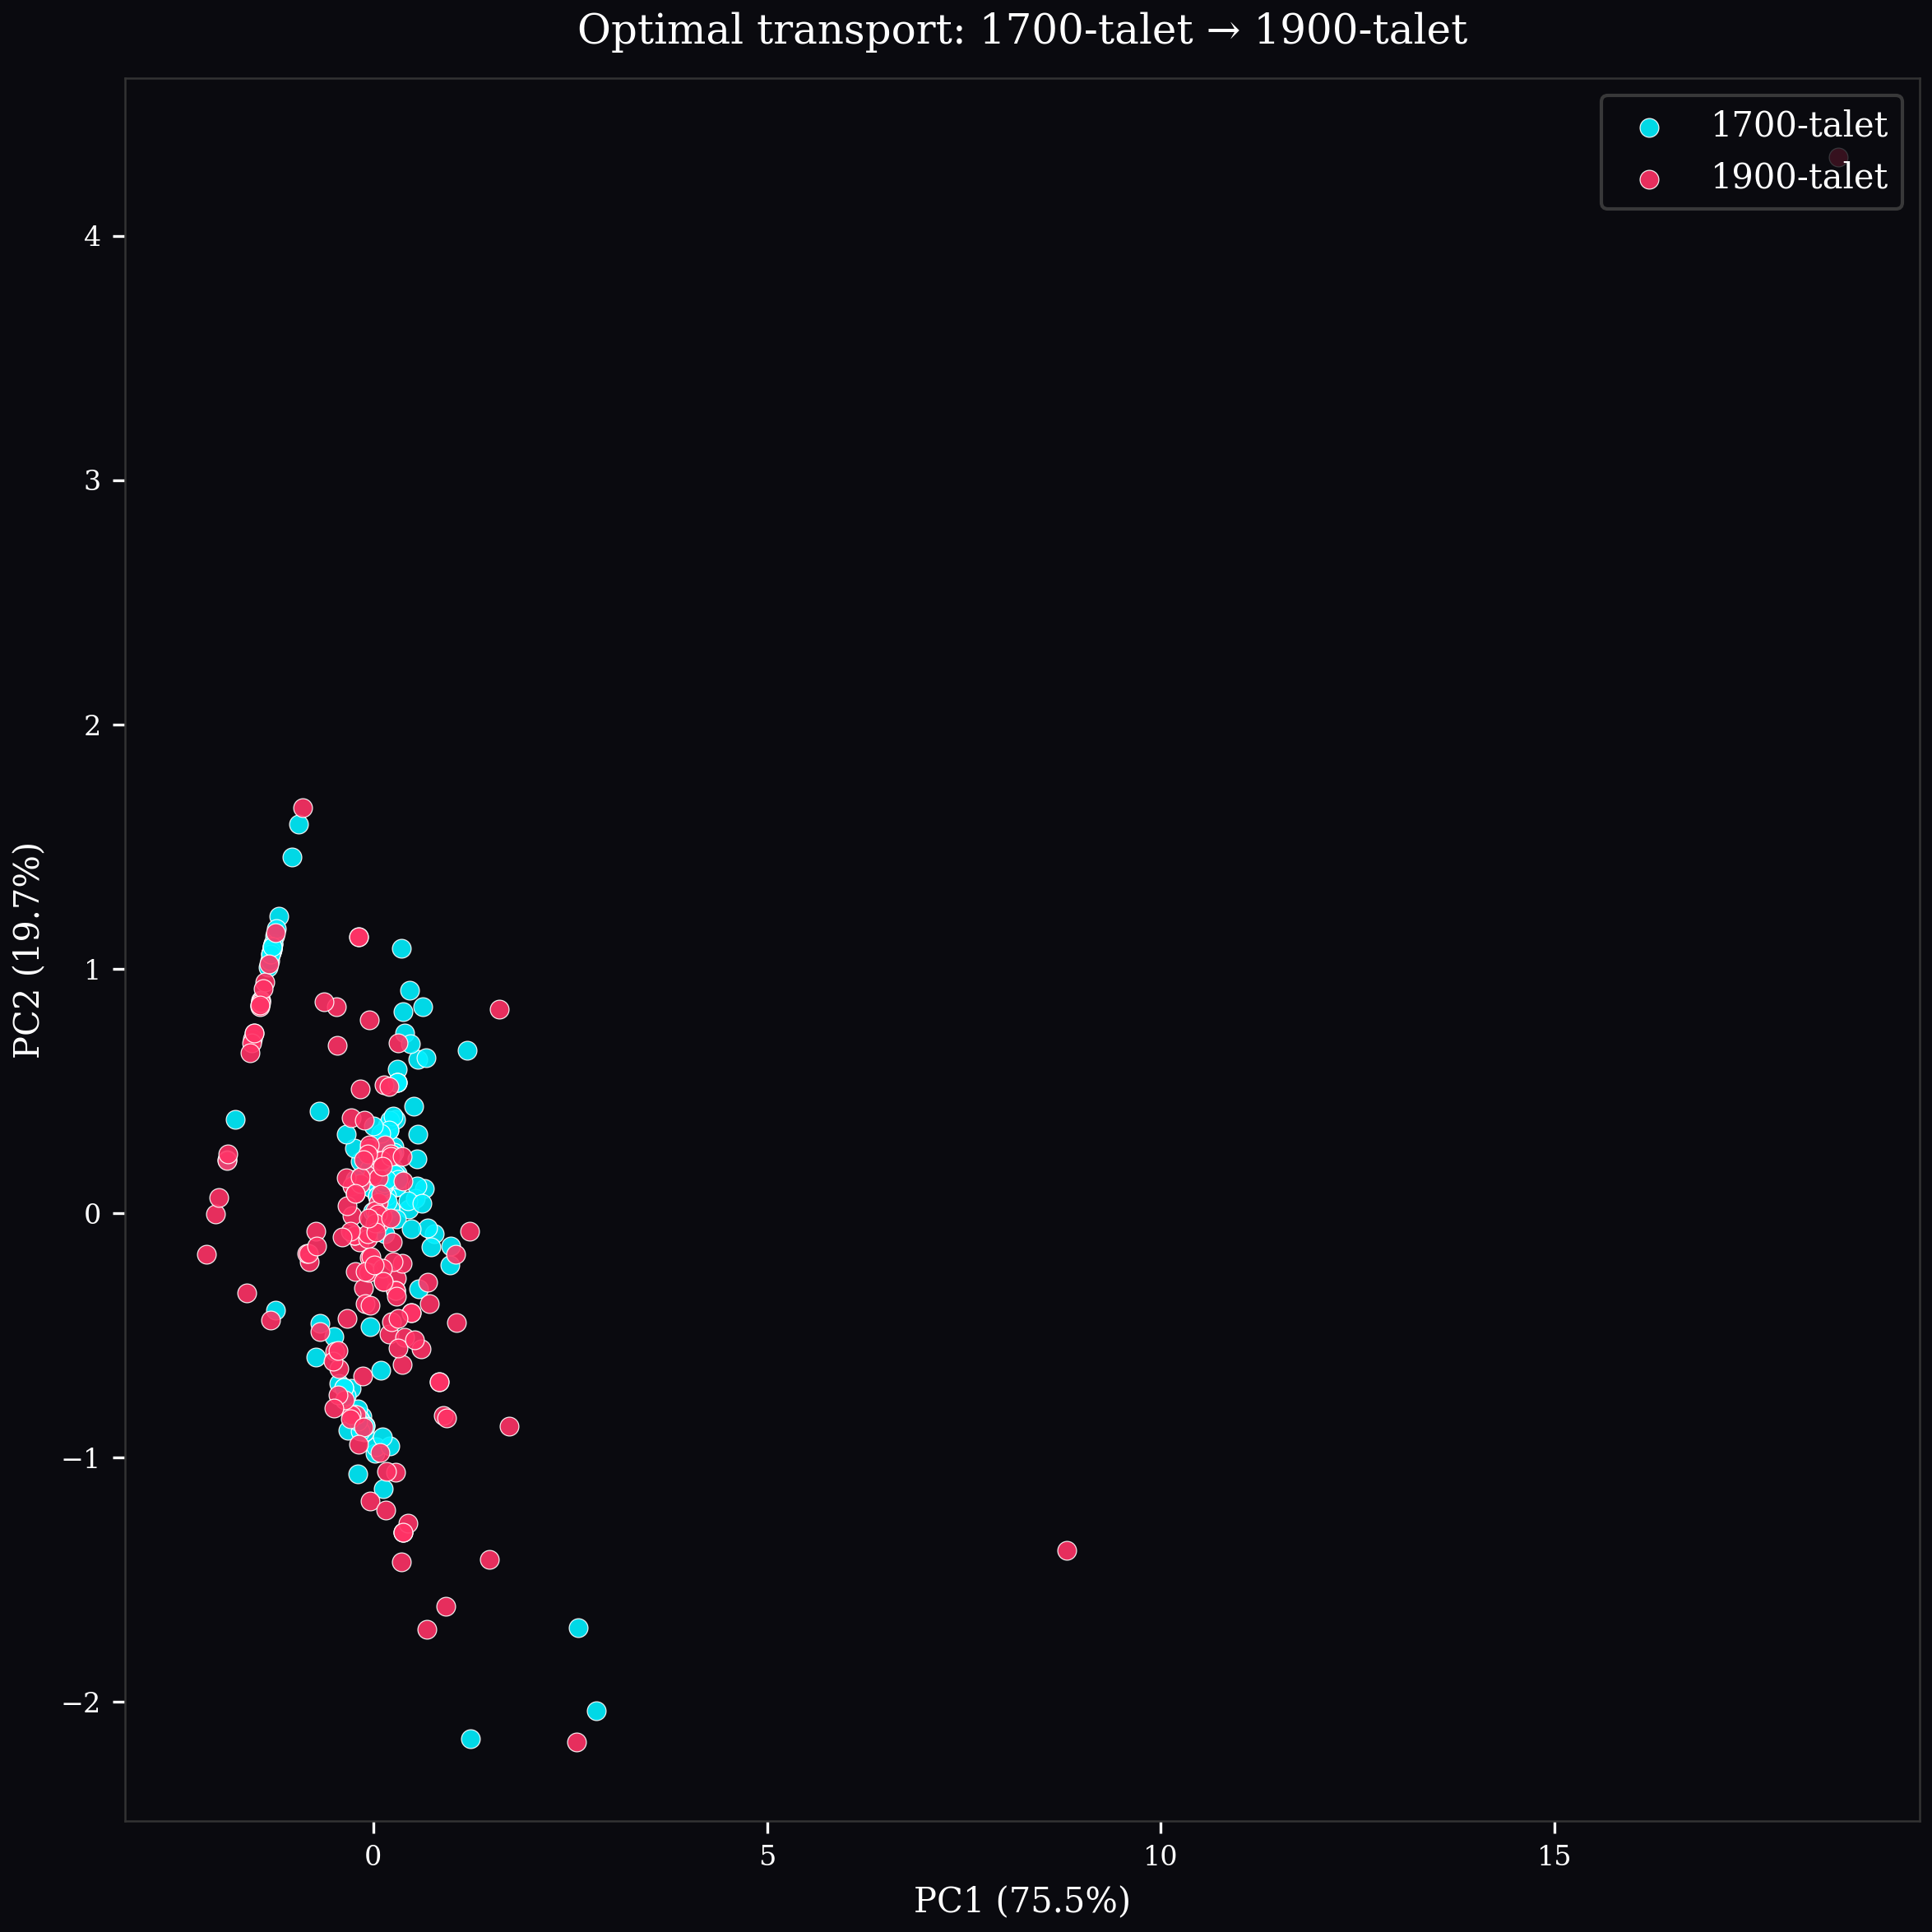
\includegraphics[width=\columnwidth]{fig6_transportplan.png}
  \caption{Optimal transport-plan mellom 1700-talet (cyan) og 1900-talet (magenta). Linjene syner dei sterkaste koplingslinene -- stolar som korresponderer i form.}
  \label{fig:transport}
\end{figure}


\subsection{Spektralanalyse av similaritetsgrafen}

Figur~\ref{fig:spektral} syner resultata fr\aa{} spektralanalysen. Panel (a) er den spektrale innleiringa (Fiedler-eigenvektoren $\phi_1$ mot $\phi_2$), farga etter \aa rstal. Innleiringa avdekkjer ein anna geometri enn UMAP: der UMAP prioriterer lokale naboskapar, fangar den spektrale innleiringa \emph{globale} separasjonar i formrommet.

Panel (b) syner eigenspektrumet. Det spektrale gapet -- differansen mellom konsekutive eigenverdiar -- indikerer kor mange \emph{naturlege klynger} formrommet har. Eit tydeleg gap etter den f\o rste eigenverdien tyder p\aa{} eit fundamentalt to-delt formrom, konsistent med det bin\ae re materialskiljet mellom organiske og uorganiske stolar.

\begin{figure*}[t]
  \centering
  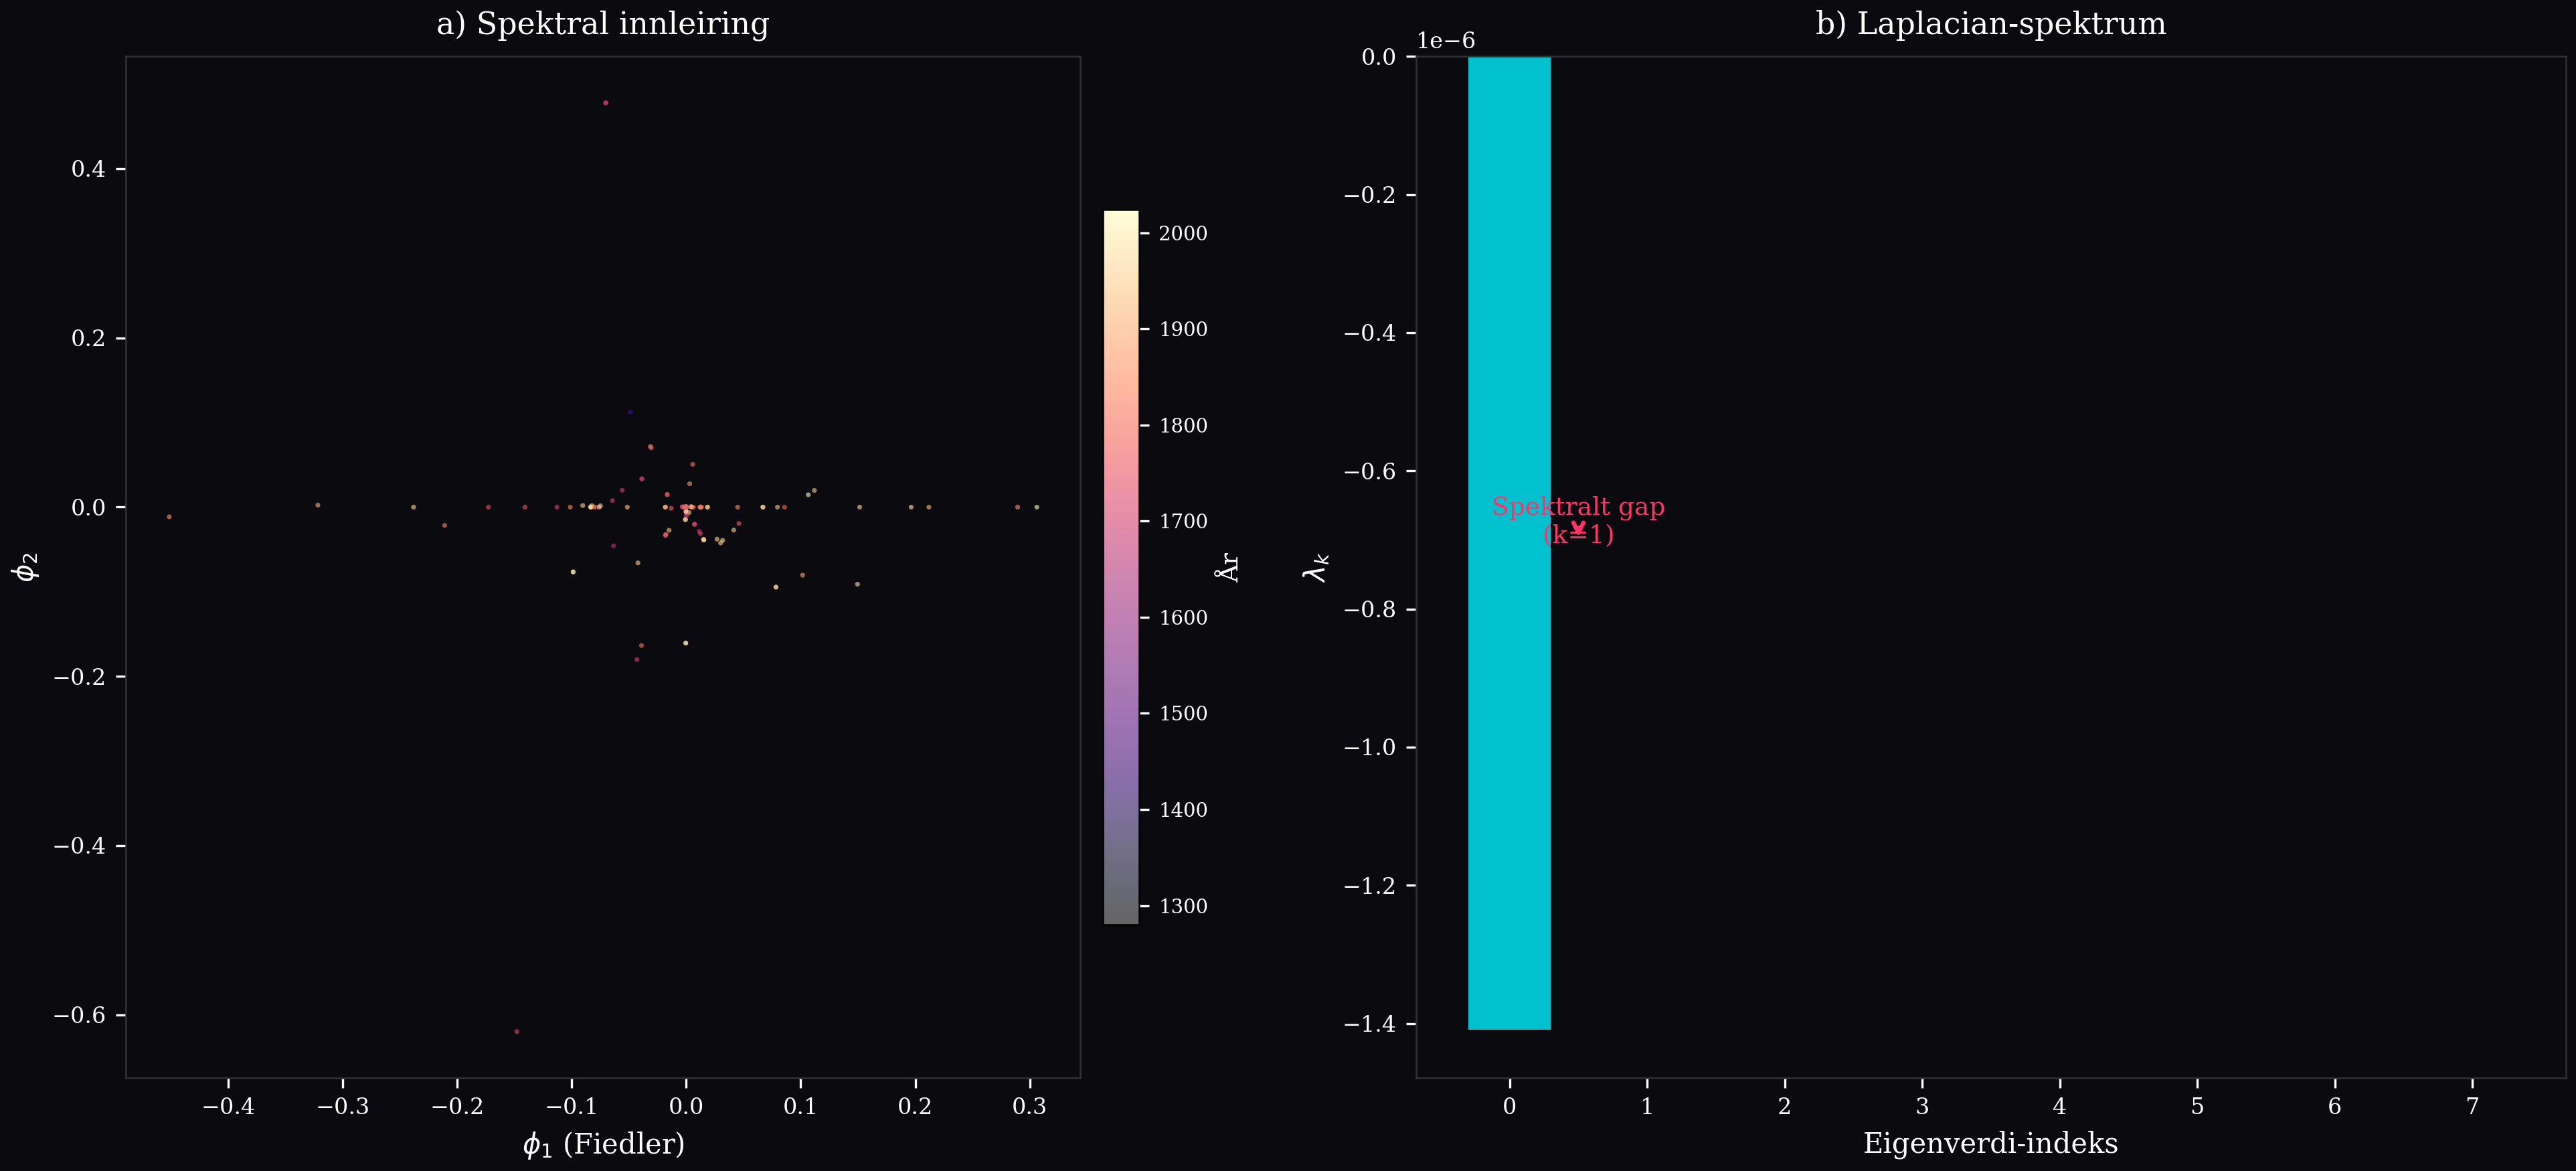
\includegraphics[width=\textwidth]{fig7_spektral.png}
  \caption{Spektralanalyse. (a) Spektral innleiring ($\phi_1$ vs.\ $\phi_2$) farga etter \aa rstal. (b) Laplacian-eigenspektrum med det spektrale gapet markert.}
  \label{fig:spektral}
\end{figure*}


\subsection{Topologisk kompleksitet over tid}

Figur~\ref{fig:persistenslandskap} syner korleis den topologiske kompleksiteten til formrommet endrar seg over hundre\aa ra. Talet p\aa{} $H_1$-trekk (l\o kker) aukar markant fr\aa{} 1500-talet til 1900-talet, medan snitt-persistensen har ein meir nyansert kurve. Tolkinga: jo fleire l\o kker formrommet har, desto fleire alternative evolusjonsvegar finst det. Det 1800-talet, med si eksplosive materialinnovasjon, har flest l\o kker -- st\o rst topologisk mangfald.

\begin{figure}[t]
  \centering
  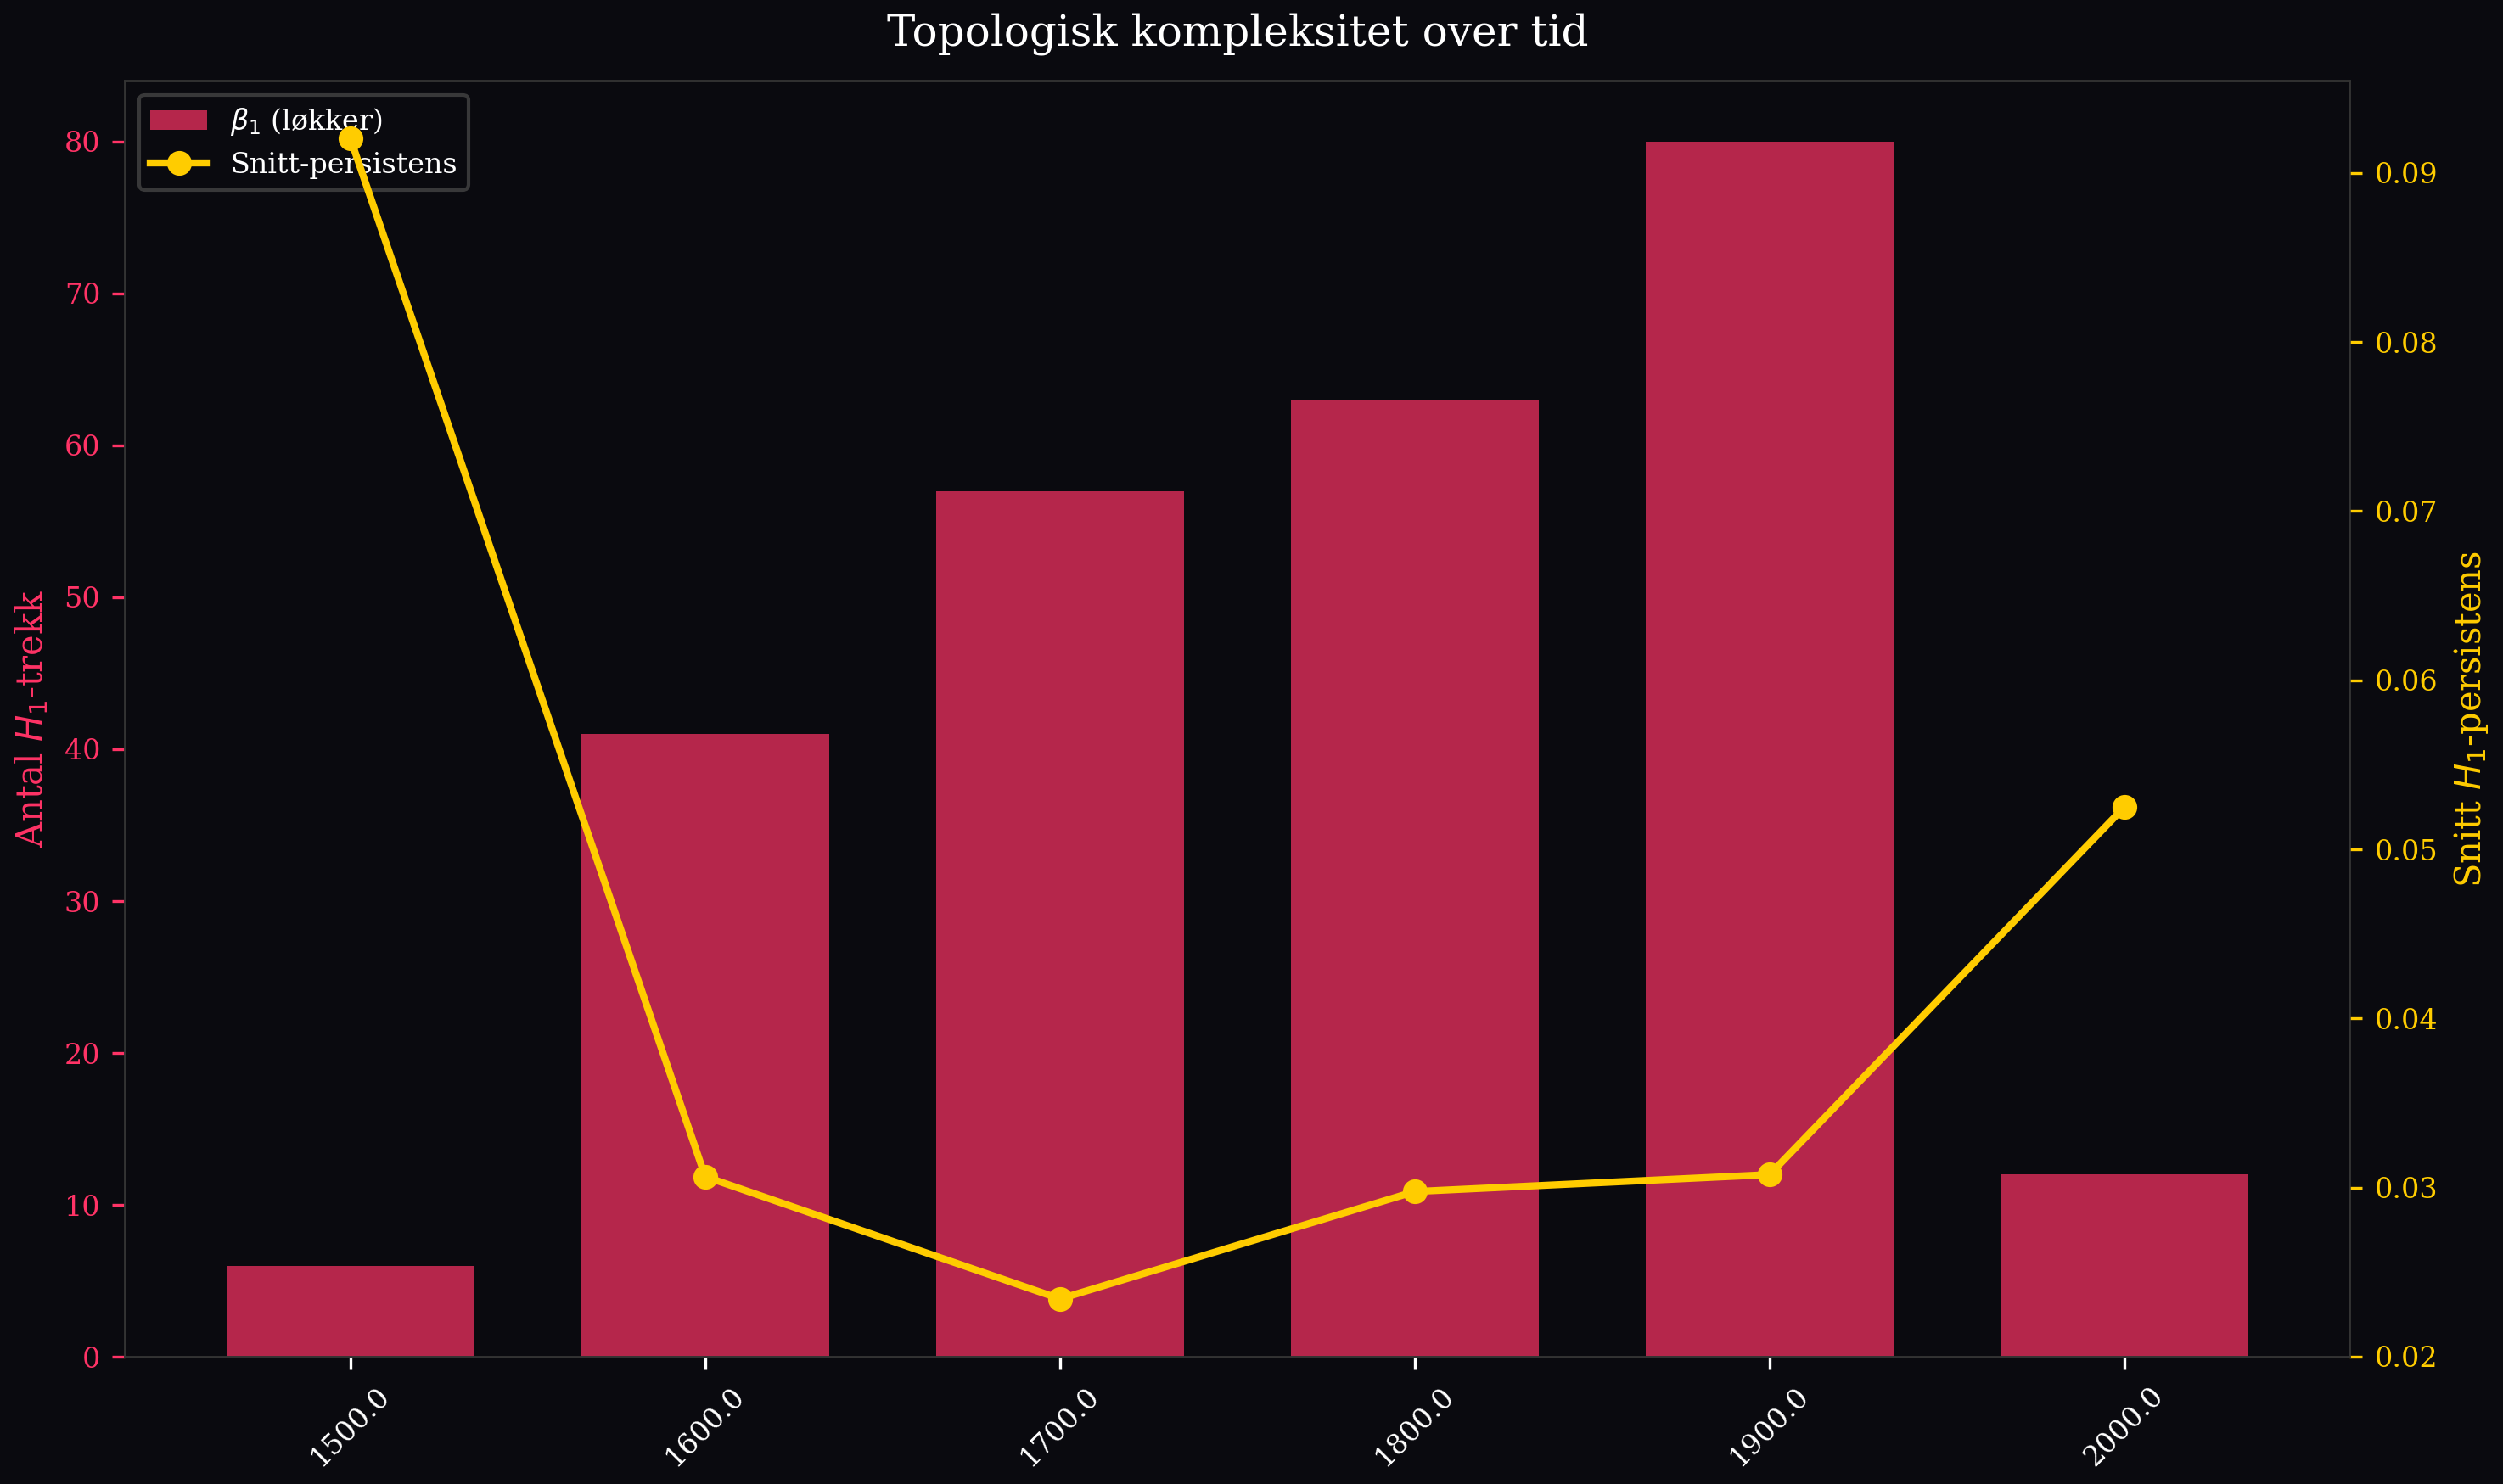
\includegraphics[width=\columnwidth]{fig8_persistenslandskap.png}
  \caption{Topologisk kompleksitet over tid. S\o yler: tal p\aa{} $H_1$-trekk (l\o kker) per hundre\aa r. Linje: snitt-persistens.}
  \label{fig:persistenslandskap}
\end{figure}


\subsection{Dimensjonell varianstunnel}

Figur~\ref{fig:varianstunnel} presenterer varians\-tunnelen: ein visualisering av korleis interkvartil- og interdecil-spreiinga i dei tre hovuddimensjonane endrar seg over 50-\aa rsperiodar. Tunnelen smalnar dramatisk etter 1800 for h\o gde, noko som tyder p\aa{} aukande \textbf{seleksjonstrykk} mot ein standardisert sitjeh\o gde. Breidde og djupn held seg meir stabile, men viser interessante lokale utvid\-ingar rundt stilovergangane.

Varianstunnelen er eit direkte m\aa l p\aa{} seleksjonstrykk: ein smal tunnel betyr sterk seleksjon (former vert tvunge mot ein standard), medan ein vid tunnel betyr svak seleksjon (stor formell fridom). Korrelasjonen mellom tunnel\-breidde og materialdiversitet (jf.\ fasediagrammet) stadfester \textbf{hypotese~H6}: volum-varians korresponderer med styrken p\aa{} seleksjonskraftene.

\begin{figure}[t]
  \centering
  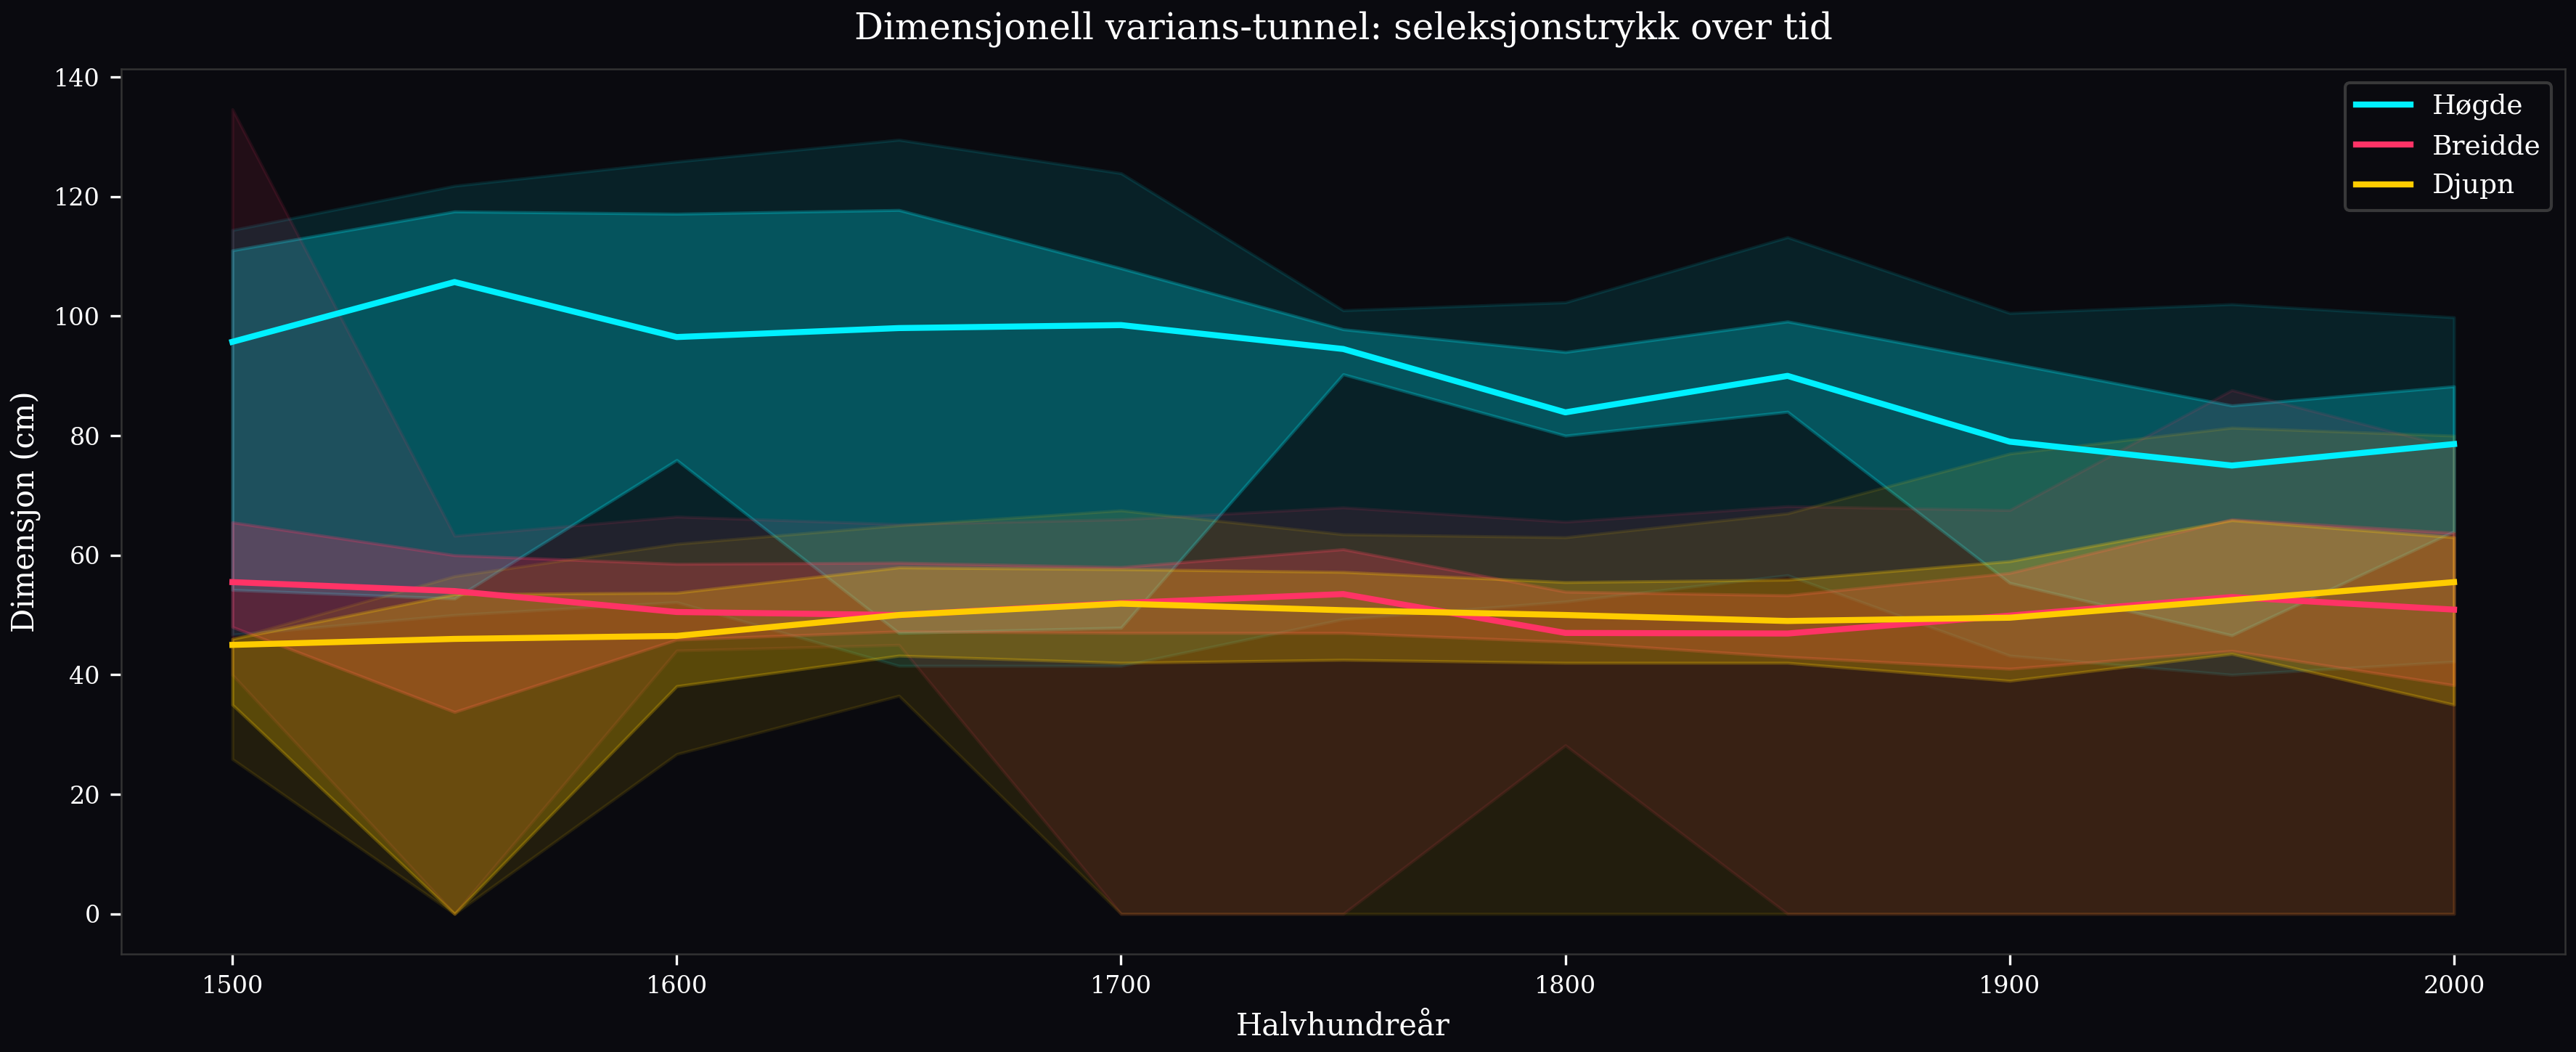
\includegraphics[width=\columnwidth]{fig9_varianstunnel.png}
  \caption{Dimensjonell varianstunnel. Skuggefelta syner 10--90-persentil (lyst) og 25--75-persentil (m\o rkt) for h\o gde, breidde og djupn over tid.}
  \label{fig:varianstunnel}
\end{figure}


\subsection{Fasediagram: materialovergangar}

Figur~\ref{fig:fasediagram} visualiserer materialfraksjonane over tid som eit stapelareal-diagram -- eit fasediagram for formrommet. Tre distinkte fasar tr\ae r fram:

\begin{enumerate}
  \item \textbf{Treepoken} (f\o r 1750): Eik, mahogni og andre tresortar dominerer totalt. Materialspektrumet er smalt; formrommet er avgrensa til det treverk tillater.
  \item \textbf{Hybridfasen} (1750--1900): Tekstil, l\ae r og polstringmaterialar kjem inn. Materialspektrumet breier seg; formrommet expanderer.
  \item \textbf{Polyfasen} (etter 1900): St\aa l, aluminium, plast, skumplast -- ein eksplosjon av nye materialar. Materialspektrumet n\aa r maksimal breidde; formrommet eksploderer i alle retningar.
\end{enumerate}

Desse fasane korresponderer n\o yaktig med dei topologiske endringane: polyfasen har flest $H_1$-l\o kker, st\o rst dimensjonell varians, og mest diffuse vektorfelt.

\begin{figure*}[t]
  \centering
  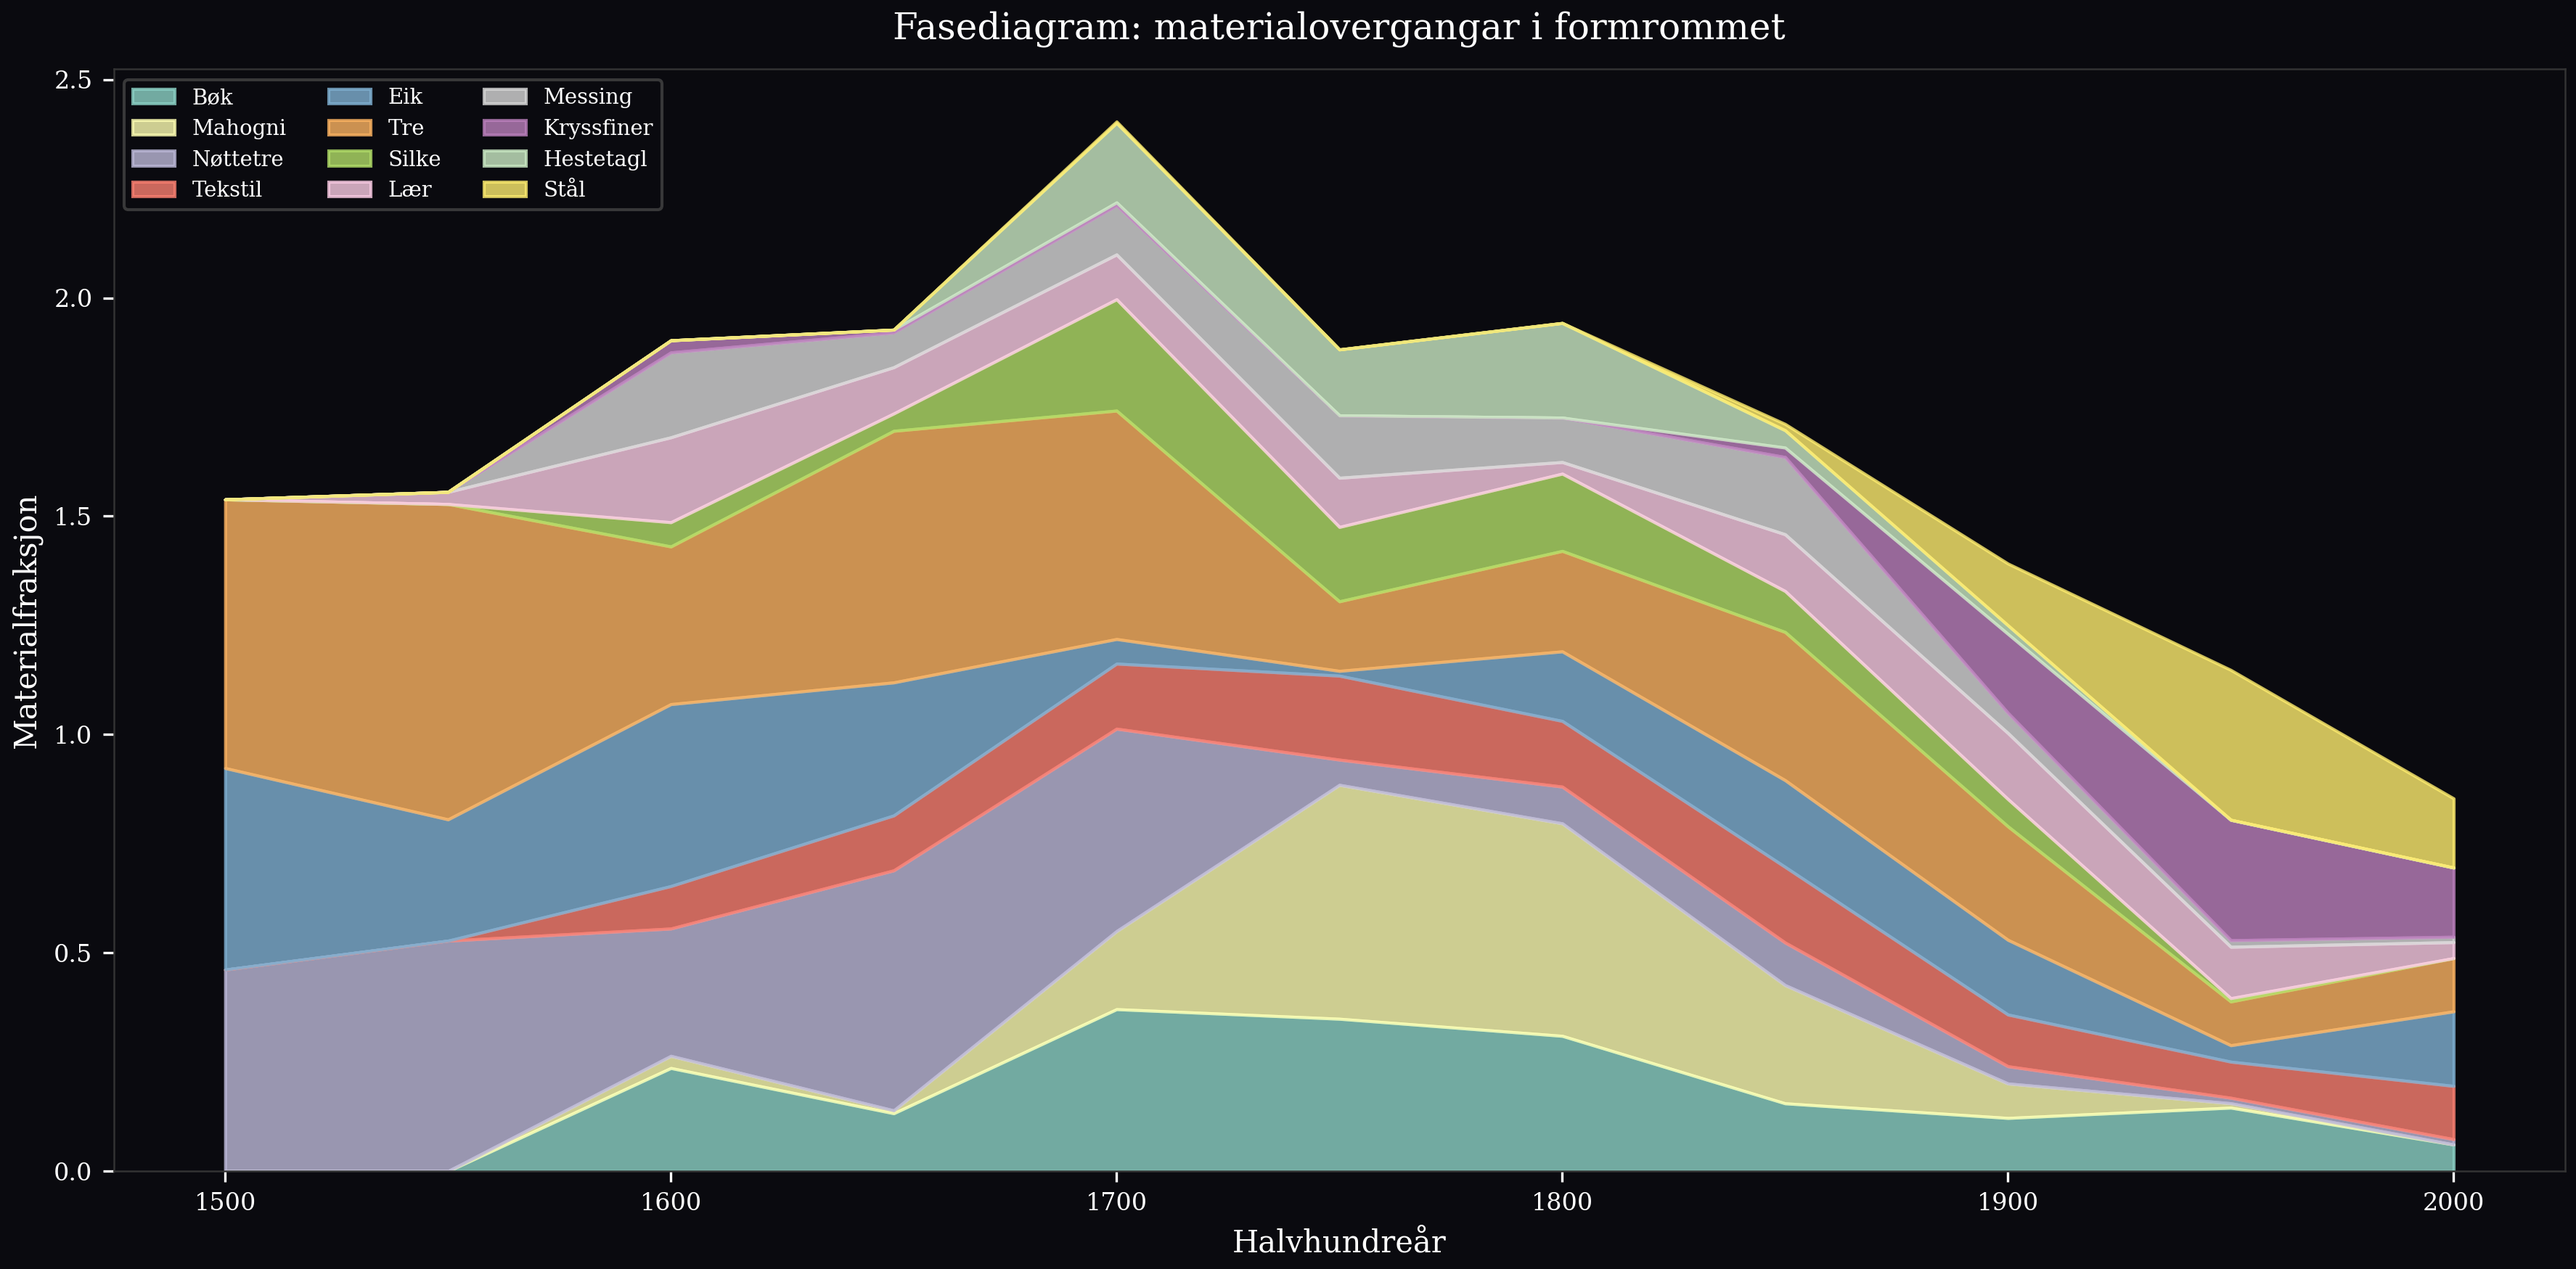
\includegraphics[width=\textwidth]{fig10_fasediagram.png}
  \caption{Fasediagram for materialovergangar. Stapelareal-diagrammet syner tre distinkte fasar: treepoken, hybridfasen og polyfasen.}
  \label{fig:fasediagram}
\end{figure*}


% ================================================================
\section{Diskusjon}
\label{sec:diskusjon}

\subsection{Seleksjonstrykk som geometri, ikkje kategori}

Det mest grunnleggjande bidraget fr\aa{} denne artikkelen er eit \emph{skift i perspektiv}: seleksjonstrykk i designhistoria b\o r ikkje forst\aa ast som diskrete kategoriar (``dette er eit materialtrykk'', ``dette er eit stilistisk trykk''), men som \textbf{geometriske eigenskapar ved formrommet}. Vektorfelta i Figur~\ref{fig:vektorfelt} og \ref{fig:ortogonal} syner at kreftene er \emph{retningar}, ikkje \emph{boksar}. Dei har styrke, retning, og dei varierer over rommet.

Denne geometriske forst\aa inga har ein viktig konsekvens: seleksjonstrykk kan vere \textbf{lokalt ortogonale men globalt korrelerte}. To krefter kan dra i same retning i \'{e}in region av formrommet og i motsett retning i ein annan. Det er denne lokale variasjonen som skaper den rike topologien me observerer -- l\o kkene, holromma, dei alternative vegane.

\subsection{Wasserstein-drifta og formens tregleik}

Eit overraskande funn er at den st\o rste Wasserstein-drifta ikkje kjem med den industrielle revolusjonen, men med renessansen. Ei mogleg forklaring er \textbf{formens tregleik}: n\aa r eit rikt mangfald av materialar og teknikkar er tilgjengelege (som i det 20.\ hundre\aa ret), kan innovasjon skje innanfor det eksisterande formrommet. Men n\aa r eit \emph{nytt} materiale kjem inn i eit \emph{smalt} formrom (som mahogni inn i det gotiske), tvingest heile fordelinga til \aa{} flytte seg.

Optimal transport gjev denne innsikta ein presis matematisk form. Wasserstein-distansen m\aa ler ikkje berre kor \emph{ulike} to fordelingar er (som KL-divergens eller Jensen-Shannon), men kor mykje \emph{arbeid} som trengst for \aa{} transformere den eine til den andre. Denne skilnaden er kritisk: to svært ulike fordelingar kan likevel vere ``n\ae re'' i Wasserstein-forstand dersom dei kan knytast saman med korte transportvegar.

\subsection{Det tomme formrommet: $H_2$ og ubrukte mogelegheiter}

Dei svake $H_2$-signala i persistensanalysen hint til eksistensen av \textbf{holrom} i formrommet: regionar som er omgjevne av realiserte former, men som sj\o lve er uutforska. Desse ``lacunae'' er ikkje tilfeldige tomrom; dei er geometrisk innkapsla mogelegheitsrom.

Fr\aa{} eit designteoretisk perspektiv er dette eit ekstraordin\ae rt funn. Det tyder p\aa{} at det finst stolar som er \emph{geometrisk plausible} -- omgjevne av eksisterande former i alle retningar -- men som aldri er produserte. Kvifor? Kanskje fordi dei ligg i ein ``blindsone'' mellom etablerte tradisjonar. Kanskje fordi dei krev ein materialkombinasjon som ikkje har vore prøvd. Uansett: TDA identifiserer desse lacunae objektivt, som potensielle m\aa l for framtidig designinnovasjon.

\subsection{Implikasjonar for designforsking}

Denne artikkelen demonstrerer at matematiske verkt\o y fr\aa{} topologi og optimal transport kan gje genuint nye innsikter i designhistoria. TDA oppdagar struktur som ikkje er synleg med tradisjonell statistikk (gjennomsnitt, varians, korrelasjonar). Optimal transport gjev eit m\aa l p\aa{} formendring som respekterer geometrien til formrommet. Saman opnar dei for ei \textbf{topologisk designhistorie}: ei forst\aa ing av formutvikling som tek p\aa{} alvor at designrommet har form, og at denne forma b\ae r informasjon.

Den viktigaste praktiske implikasjonen er for \textbf{generativ design}: dersom formrommet har identifiserbare holrom, kan desse brukast som m\aa l for algoritmisk utforsking. Optimal transport-planar mellom ulike periodar kan inspirere nye designprosessar der ein systematisk ``interpolerer'' mellom historiske tradisjonar.


% ================================================================
\section{Konklusjon}
\label{sec:konklusjon}

Denne artikkelen har, for f\o rste gong, brukt topologisk dataanalyse og optimal transport p\aa{} ei stor designhistorisk samling. Hovudfunna er:

\begin{enumerate}
  \item Formrommet til europeiske stolar har ikkje-trivielle topologiske trekk: $H_0$-klynger som korresponderer med materialdomene, $H_1$-l\o kker som reflekterer sykliske evolusjonsvegar, og $H_2$-antydningar til uutforska regionar.
  \item Wasserstein-drifta avsl\o rer at den st\o rste formtransformasjonen skjedde med renessansen ($W_1 = 1{,}56$), ikkje med den industrielle revolusjonen.
  \item Seleksjonstrykk opererer som delvis ortogonale vektorfelt p\aa{} formrommet -- tid, material og dimensjonar dreg i ulike retningar.
  \item Formrommet gjennomg\aa r tre distinkte materialfasar: treepoken, hybridfasen og polyfasen, kvar med ulik topologisk kompleksitet.
\end{enumerate}

Saman peikar desse funna mot ei ny forst\aa ing av designevolusjonen: ikkje som ein line\ae r progresjon, men som ein topologisk rik vandring gjennom eit mangfaldig formrom -- forma av krefter som dreg i ulike retningar, og som opnar og lukkar mogelegheiter etter kvart som nye materialar og teknikkar vert tilgjengelege.


% ================================================================
\bibliographystyle{plainnat}
\bibliography{references}

\end{document}
